\chapter{A Dictionary Language}
\label{chap:A-Dictionary-Language}

When establishing a model-driven solution, \emph{model transformations} usually play a central and important role.
\marginpar{\emph{A Taxonomy of Model Transformations}}
Be it for specifying dynamic semantics (like for our learning box) or, more generally, for transforming a certain model to another model to achieve some goal (consistency, adding or abstracting from platform details, \ldots).  

There are many \emph{types} of model transformations and \cite{CH03,Mens_Gorp_2006} give a nice and detailed classification along a set of different dimensions. 
\marginpar{\emph{Model-to-Text\\ Transformations}}
In this chapter, we shall explore some of these dimensions and learn how \emph{model-to-text} transformations can be achieved with a nice mixture of \emph{string grammars} and \emph{graph grammars}. 

For the rest of the chapter a model transformation is to be regarded as:
\begin{displaymath}
 	\Delta: m_{src} \rightarrow m_{trg}
\end{displaymath}
where the source model $m_{src}$ is to be transformed to the target model $m_{trg}$.

$\Delta$ is \emph{endogenous}, if $m_{src}$ and $m_{trg}$ conform to the same metamodel.
\marginpar{\emph{Endogenous Model\\ Transformations}}
All the SDMs we have treated in the tutorial till now (for our learning box) are examples of endogenous transformations.

$\Delta$ is \emph{exogenous}, if $m_{src}$ and $m_{trg}$ are instances of different metamodels.
\marginpar{\emph{Exogenous Model\\ Transformations}}
In this chapter, we shall complement our learning box with a simple language for \emph{dictionaries}.
A dictionary is also used to learn new words but is more suitable to be used as a reference, i.e., one already knows most of the words and only specific words are looked-up now and then.
A learning box, on the other hand, is more geared towards supporting the actual memorization process.
Ergo?  One could start with a learning box and, when all words have been memorized, transform it to a personalized dictionary for future reference.
If one notices that too many words have been forgotten (typically after a long break or a lazy spell) a dictionary can be transformed \emph{back} to a learning box.
We shall see later on that this transformation is actually quite cool as one could, for example, use the history of cards or their difficulty level (fast cards are very simple) to either annotate entries in a dictionary or pre-place cards appropriately in a learning box. 

The learning box to dictionary transformation and vice-versa are examples of exogenous transformations.

$\Delta$ operates \emph{in-place}, if $m_{src}$ is destructively transformed to $m_{trg}$.
\marginpar{\emph{In-Place Model\\ Transformations}}
The SDMs for our learning box (e.g. grow or check) are examples for in-place transformations as they perform changes directly to a source model, transforming it destructively into the target model.


$\Delta$ is \emph{out-place} if $m_{src}$ is left intact and is not changed by the transformation that creates $m_{trg}$.
\marginpar{\emph{Out-Place Model\\ Transformations}}
The learning box to dictionary transformation and vice-versa are examples of out-place transformations.

Although endogenous + in-place is the natural case for SDMs (like for our learning box), we shall see in a moment that exogenous and/or out-place transformations can also be specified with SDMs.

%\vspace{1.5cm}
 
To twist your brain a bit here are a few interesting statements:
\begin{enumerate}
\item[$\blacktriangleright$] Out-place transformations can be endogenous or exogenous.

\item[$\blacktriangleright$] In-place transformations can usually\footnote{One can always think up crazy examples right?} only be endogenous.  Exogenous transformations are, consequently, always out-place.  Why? 
\end{enumerate}  

%\vspace{1.5cm}
   
$\Delta$ is further classified as \emph{horizontal} if $m_{src}$ and $m_{trg}$ are on the same \emph{abstraction level} and \emph{vertical} if they are not. 
\marginpar{\emph{Horizontal or\\ Vertical?}}

This last abstraction-level dimension is unfortunately a bit fuzzy but in a moment we shall explore and work on 
\marginpar{\emph{Abstraction Levels}}
different abstraction levels by establishing a textual concrete syntax for our dictionaries.

In the process we shall learn how graph transformations can be used, in combination with parser generators and template languages, to implement model-to-text and text-to-model transformations that are typically vertical (text is normally on a lower abstraction level than a model).  

Our learning box to dictionary transformation is, on the other hand, probably horizontal as the models represent the \emph{same} information, albeit differently, and can thus be considered to be on the same abstraction level.

\vspace{1.5cm}


In the following the \emph{Mo}flon \emph{C}ode \emph{A}dapter (\emph{Moca}) framework refers to:
\begin{enumerate}
 \item the approach we use to integrate string grammars, graph grammars and template languages, 
 \item how we separate the transformation into different modular steps, 
\marginpar{\emph{What is Moca?}}
 \item the usage of a generic and simple tree to consolidate different platforms, and 
 \item the actual tool support that acts as glue to hold all the different parts together.
\end{enumerate}
 
Fig.~\ref{fig:moca-overview} gives a ``big picture'' of what we plan to achieve in this chapter.
All explanations are integrated right in the figure so take your time and let it sink in.
We'll be zooming in on bits and pieces in the following sections to make things clearer and more concrete.
%\usepackage{graphics} is needed for \includegraphics
\begin{figure}[htp]
\begin{center}
 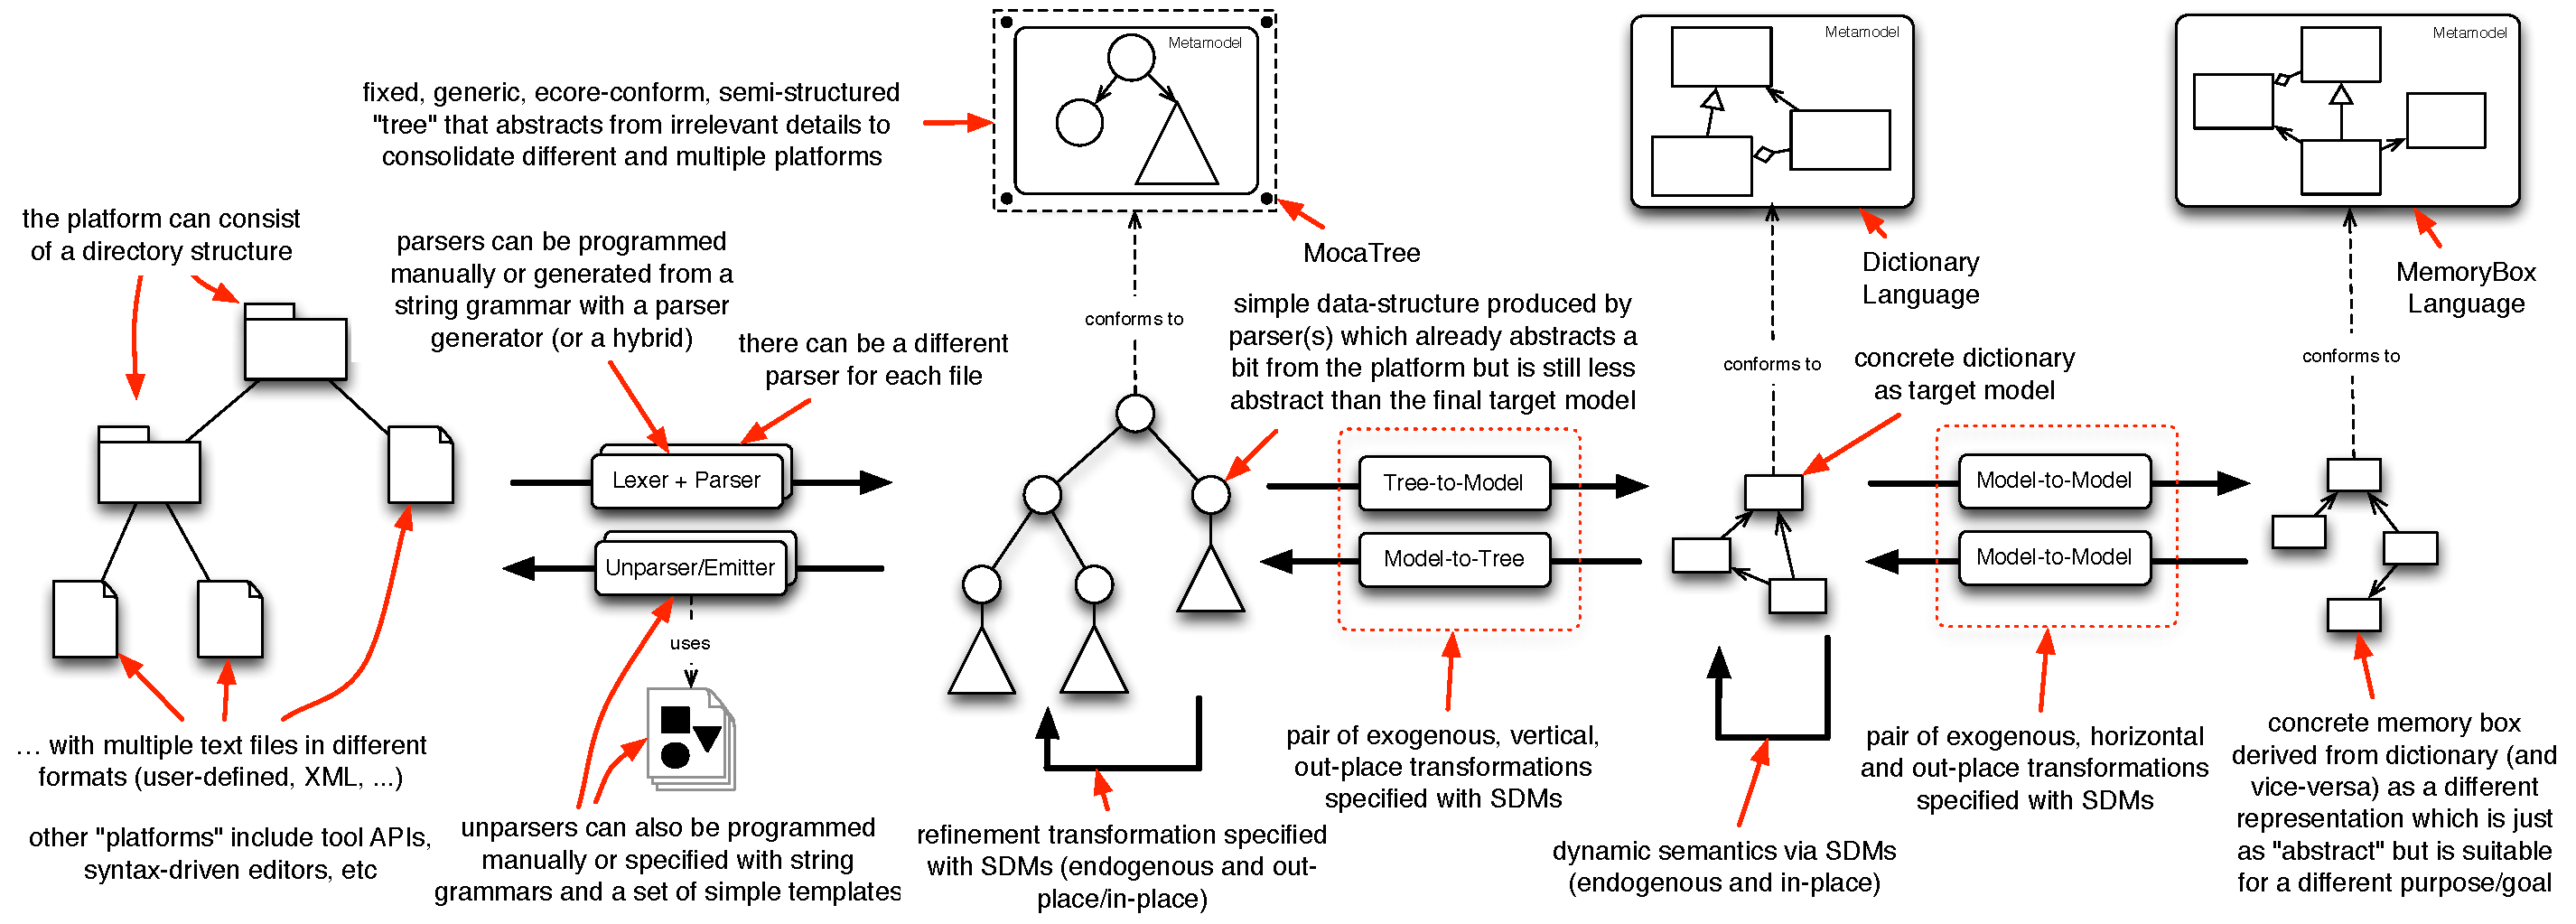
\includegraphics[angle=90, height=\textheight]{pics/moca/text-to-model}
  \caption{Overview of model-to-text with the MOCA framework}
  \label{fig:moca-overview}
\end{center}
\end{figure} 

\section{Set up ANTLR}
 
Our first step will be to install and set up a \emph{parser generator}.
Nowadays, \emph{no one} really writes a complex parser completely by hand.
Although this is sometimes still necessary\footnote{Some languages are syntactically quite challenging.} most parsers can be whipped up pretty quickly using context-free \emph{string grammars}\footnote{For simple cases, \emph{regular expressions} can also be used.} typically in EBNF\footnote{Extended Backus-Naur Form}.
ANTLR~\cite{ANTLR} is a tool that can generate a parser from a compact EBNF specification for a host of target programming languages, including Java.
Although ANTLR might not be the most efficient or powerful parser generator out there, it is open-source, well documented and supported, and allows for a pragmatic and quite elegant \emph{fallback} to Java when things get nasty and we have to resort to some dirty tricks.

\begin{enumerate}
\item[$\blacktriangleright$] Install the ANTLR-IDE\footnote{\url{http://antlrv3ide.sourceforge.net/}} Eclipse plugin from:\\ \url{http://antlrv3ide.sourceforge.net/updates}.

We suggest you use ANTLR-IDE as it integrates nicely with eMoflon (the same build function for generating code also triggers the parser generator) and offers adequate editor functionality.

\item[$\blacktriangleright$] Download ANTLRWorks from:\\ \url{www.antlr.org/download/antlrworks-1.4.3.jar}.

ANTLRWorks\footnote{\url{http://www.antlr.org/works/index.html}} is the IDE recommended by \cite{ANTLR}.  
It offers a nice debugger and visualization of parse trees and abstract syntax trees.
You are free to use ANTLRWorks either together with ANTLR-IDE or as an alternative.
For all screenshots and explanations, however, we shall assume you choose to work with ANTLR-IDE.  

Now choose \texttt{Directory} and browse to the directory with the downloaded ANTLRWorks jar file (Fig.~\ref{moca-2-choose-path-to-jar}).

\item[$\blacktriangleright$] Configure ANTLR for Eclipse:\\ Go to ``Window/Preferences/ANTLR/Builder'' and choose \texttt{Add} as depicted in Fig.~\ref{moca-1-antlr-package}.

As ANTLR-IDE does not provide the actual jars for the parser generator, these have to be downloaded and referenced from the plugin.
%\usepackage{graphics} is needed for \includegraphics
\begin{figure}[!htbp]
\begin{center}
 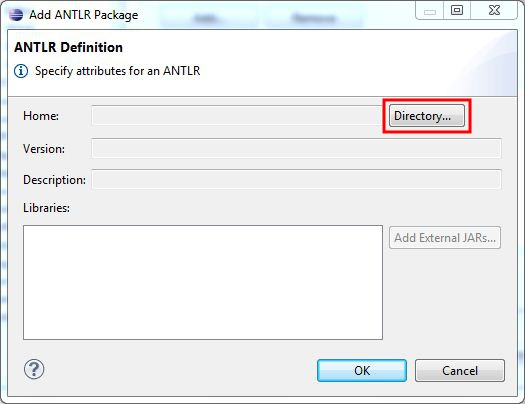
\includegraphics[width=0.8\textwidth]{pics/moca/0Install/2-choose-path-to-jar}
  \caption{Dialogue for choosing ANTLRWorks as Builder}
  \label{moca-2-choose-path-to-jar}
\end{center}
\end{figure}
%\usepackage{graphics} is needed for \includegraphics
\begin{figure}[!htbp]
\begin{center}
 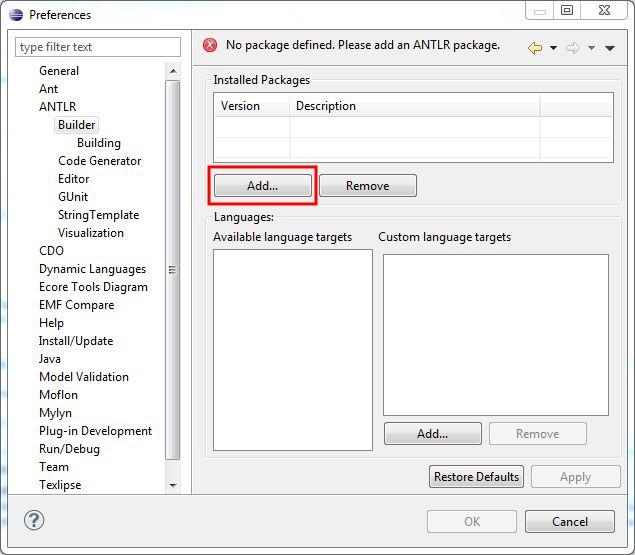
\includegraphics[width=0.8\textwidth]{pics/moca/0Install/1-antlr-package}
  \caption{Builder Preferences for ANTLR IDE}
  \label{moca-1-antlr-package}
\end{center}
\end{figure}
\end{enumerate}

\clearpage

\section{Setting up your M2T workspace}

Nowadays, \emph{no one} really writes a complex parser completely by hand.
Although this is sometimes still necessary\footnote{Some languages are syntactically quite challenging.} most parsers can be whipped up pretty quickly using context-free \emph{string grammars}\footnote{For simple cases, \emph{regular expressions} can also be used.} typically in EBNF\footnote{Extended Backus-Naur Form}.
ANTLR~\cite{ANTLR} is a tool that can generate a parser from a compact EBNF specification for a host of target programming languages, including Java.
Although ANTLR might not be the most efficient or powerful parser generator out there, it is open-source, well documented and supported, and allows for a pragmatic and quite elegant \emph{fallback} to Java when things get nasty and we have to resort to some dirty tricks.

The first step is preparing an Eclipse workspace according to our suggested workflow.

\begin{enumerate}
\item[$\blacktriangleright$] In Eclipse (preferably with an empty workspace), switch to our Moflon perspective and invoke the \texttt{New Metamodel} wizard (Fig.~\ref{fig:moca-1-NewMetamodelWizard}). 

%\usepackage{graphics} is needed for \includegraphics
\begin{figure}[!htbp]
\begin{center}
 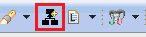
\includegraphics[width=0.3\textwidth]{pics/moca/1DictionaryMetaModel/1-NewMetamodelWizard.png}
  \caption{Invoking the \texttt{New Metamodel} wizard.}
  \label{fig:moca-1-NewMetamodelWizard}
\end{center}
\end{figure}

\item[$\blacktriangleright$] Choose ``Dictionary'' as project name and select \texttt{Add eMoflon languages} as depicted in Fig.~\ref{fig:moca-2-AddMocaSupport-ProjectName}. 

%\usepackage{graphics} is needed for \includegraphics
\begin{figure}[!htbp]
\begin{center}
 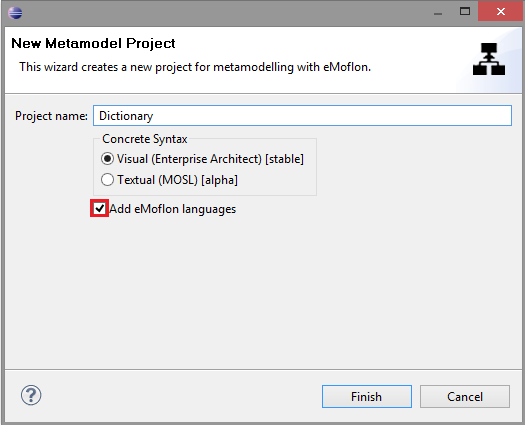
\includegraphics[width=0.7\textwidth]{pics/moca/1DictionaryMetaModel/2-AddMocaSupport-ProjectName.png}
  \caption{Add Metamodel project with MOCA support}
  \label{fig:moca-2-AddMocaSupport-ProjectName}
\end{center}
\end{figure}

\item[$\blacktriangleright$] After the project is created as usual (Fig. \ref{fig:moca-3-NewWizardResult}) double-click the EAP file to open it. 

%\usepackage{graphics} is needed for \includegraphics
\begin{figure}[!htbp]
\begin{center}
 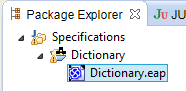
\includegraphics[width=0.3\textwidth]{pics/moca/1DictionaryMetaModel/3-WizardResult.png}
  \caption{Eclipse workspace after creating the \texttt{Dictionary} project}
  \label{fig:moca-3-NewWizardResult}
\end{center}
\end{figure}

\item[$\blacktriangleright$] In EA, the project is already populated with the metamodel for our generic tree.
To differentiate this from other trees (ANTLR parse tree and abstract syntax tree, XML DOM tree, \ldots) we shall refer to it as \texttt{MocaTree} (Fig.~\ref{fig:moca-4-eapContainsMocatreeWithExportFalse}).
Note that the \texttt{MocaTree} package has a special tagged value \texttt{Moflon::Export} that is set to \texttt{false}\footnote{Tagged values can be viewed in the \texttt{Tagged Values} view in EA (Fig.~\ref{fig:moca-4-eapContainsMocatreeWithExportFalse}).}.
This ensures that the package is \emph{ignored} when exporting.
As with all standard metamodels (e.g., Ecore or the SDM metamodel) the \texttt{MocaTree} package in EA should be regarded as read-only and is only required in the EA project so that SDMs can refer to the classes defined in the package.
The corresponding Java code is provided by our Eclipse plugin and is added automatically to the Java build path whenever necessary.

%\usepackage{graphics} is needed for \includegraphics
\begin{figure}[!htbp]
\begin{center}
 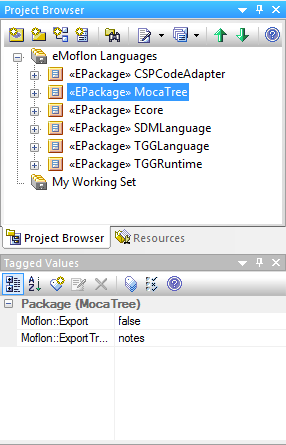
\includegraphics[width=0.4\textwidth]{pics/moca/1DictionaryMetaModel/4-eapContainsMocatreeWithExportFalse.png}
  \caption{\texttt{MocaTree} in default EA project}
  \label{fig:moca-4-eapContainsMocatreeWithExportFalse}
\end{center}
\end{figure}
\end{enumerate}

Go ahead and inspect the \texttt{MocaTree} metamodel (Fig.~\ref{fig:moca-tree}).
It basically combines concepts from a filesystem (folders and files), XML concepts (text-only nodes and attributes), and a general indexed\footnote{The index attribute in \texttt{TreeElement} can be used to demand a certain \emph{order} of nodes in an SDM, which is otherwise not guaranteed by default (order is in general non-deterministic).} containment hierarchy.

\begin{figure}[!htbp]
\begin{center}
 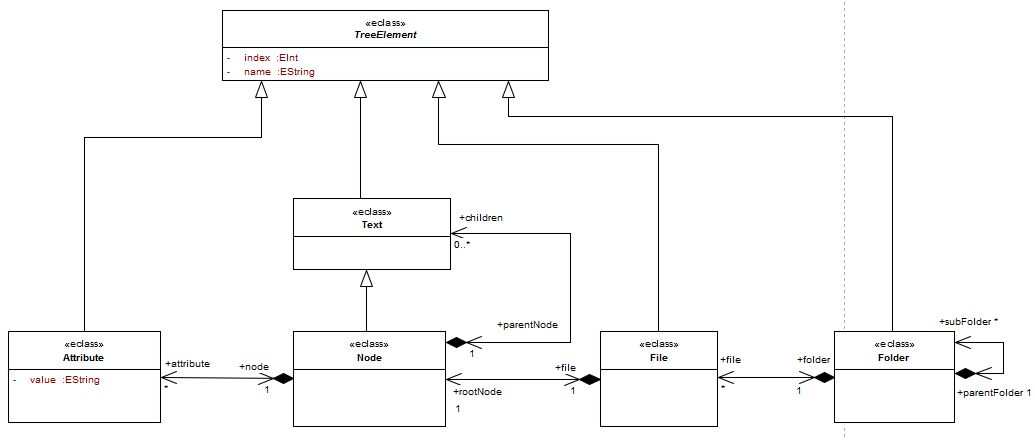
\includegraphics[width=\textwidth]{pics/moca/0Install/0-MocaTree}
  \caption{\texttt{Mocatree} Metamodel}
  \label{fig:moca-tree}
\end{center}
\end{figure}
 
\begin{enumerate}

\item[$\blacktriangleright$] Add a new package \texttt{DictionaryLanguage} and model the required classes and relationships for our dictionary language (Fig.~\ref{fig:moca-5-DictionaryMM}).

Every dictionary has a title and consists of entries.
Entries have a content and a level that indicates how difficult the entry is.
Dictionaries can be organized in shelves that have a description and shelves can be collected in a library.
To make things interesting, each dictionary has an author.
Note that arbitrary many different dictionaries, irrespective of their shelves, can share the same author.

%\usepackage{graphics} is needed for \includegraphics
\begin{figure}[!htbp]
\begin{center}
 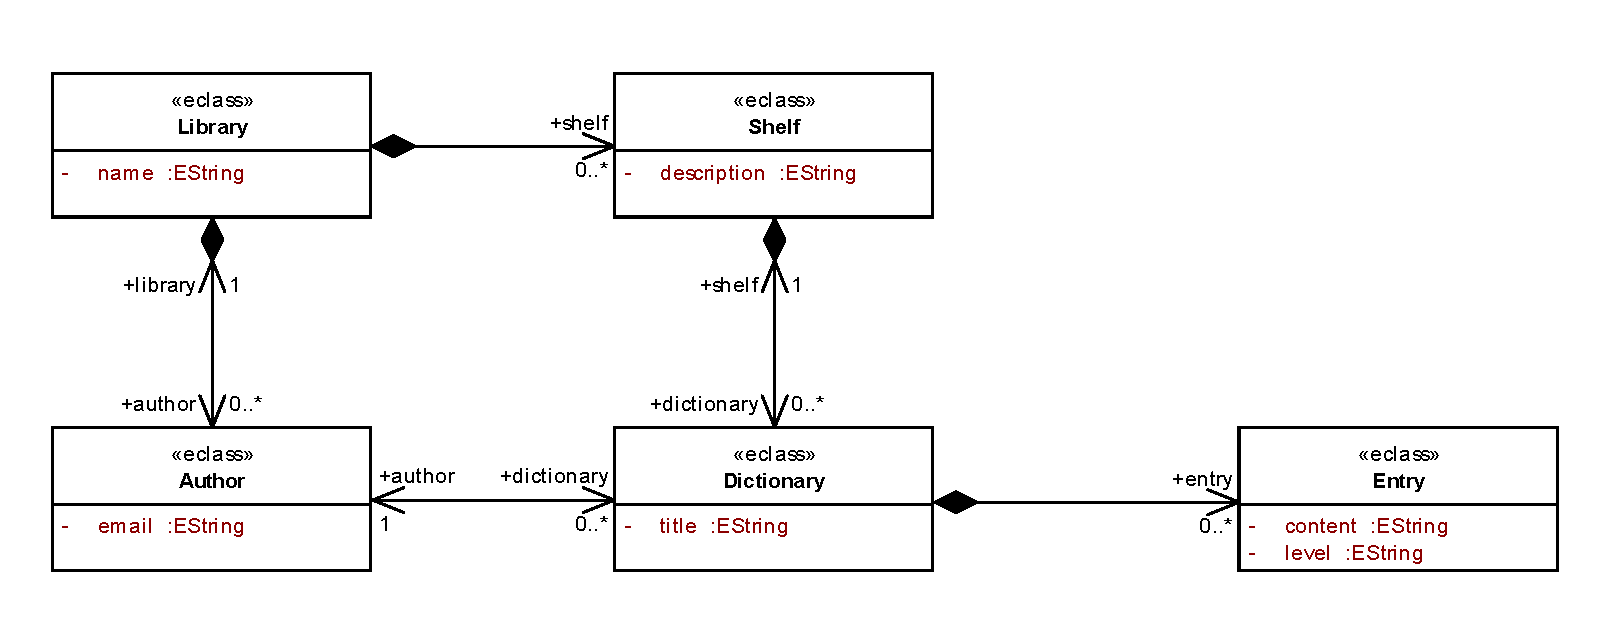
\includegraphics[width=\textwidth]{pics/moca/1DictionaryMetaModel/DictionaryLanguage}
  \caption{Dictionary Metamodel}
  \label{fig:moca-5-DictionaryMM}
\end{center}
\end{figure}

\item[$\blacktriangleright$] For the moment, add an empty package in EA named \texttt{Dic\-tion\-ary\-Code\-Adapter} so that your EA workspace closely resembles Fig.~\ref{fig:moca-5-DictionaryMM-ProjectBrowser}.

According to our conventions and workflow, a \emph{code adapter} is a package that contains the tree-to-model transformation logic.
This could of course be integrated directly in the corresponding metamodel (\texttt{Dic\-tion\-ary\-Language} in our case), but a separation makes sense as there could be \emph{different} code adapters for the \emph{same} language.
\clearpage

%\usepackage{graphics} is needed for \includegraphics
\begin{figure}[!htbp]
\begin{center}
 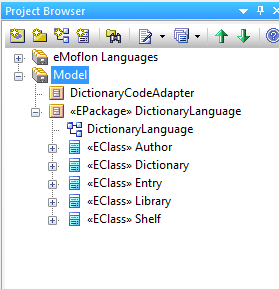
\includegraphics[width=0.4\textwidth]{pics/moca/1DictionaryMetaModel/5-DictionaryMM-ProjectBrowser.png}
  \caption{EA workspace before exporting}
  \label{fig:moca-5-DictionaryMM-ProjectBrowser}
\end{center}
\end{figure}

\item[$\blacktriangleright$] Export as usual and ensure that your Eclipse workspace closely resembles Fig.~\ref{fig:moca-6-ExportToEclipse}.
Note especially the library nodes (\texttt{Moflon} and \texttt{Moca}) that reference jars for all required dependencies. (If your \texttt{Dictionary\-Code\-Adapter} is not exported or you receive an error message while exporting it, you can add an empty diagram to it)

%\usepackage{graphics} is needed for \includegraphics
\begin{figure}[!htbp]
\begin{center}
 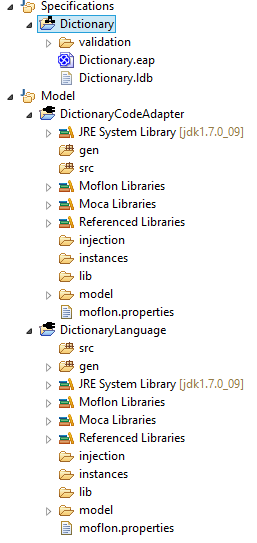
\includegraphics[width=0.4\textwidth]{pics/moca/1DictionaryMetaModel/6-ExportToEclipse.png}
  \caption{Workspace after export to Eclipse}
  \label{fig:moca-6-ExportToEclipse}
\end{center}
\end{figure}

\item[$\blacktriangleright$] Right-click on \texttt{DictionaryCodeAdapter} one more time and choose ``Add Parser/Unparser'', this time from the eMoflon context menu (Fig \ref{fig:moca-1-AddParserAndUnparserWizard}).

%\usepackage{graphics} is needed for \includegraphics
\begin{figure}[!htbp]
\begin{center}
 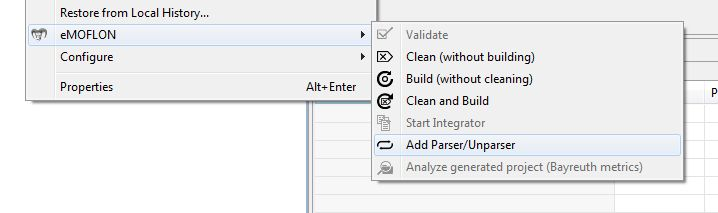
\includegraphics[width=0.75\textwidth]{pics/moca/2TextToMocaTree/1-AddParserAndUnparserWizard}
  \caption{Invoking the \texttt{Add Parser/Unparser} wizard} 
  \label{fig:moca-1-AddParserAndUnparserWizard}
\end{center}
\end{figure}
 
\item[$\blacktriangleright$] In the wizard dialogue (Fig \ref{fig:moca-2-AddParser}), enter ``dictionary'' as file extension, and check the boxes \texttt{Create Parser} and \texttt{Create Unparser} with \texttt{ANTLR} chosen as corresponding technology in both cases.  Click \texttt{Finish}. 

%\usepackage{graphics} is needed for \includegraphics
\begin{figure}[!htbp]
\begin{center}
 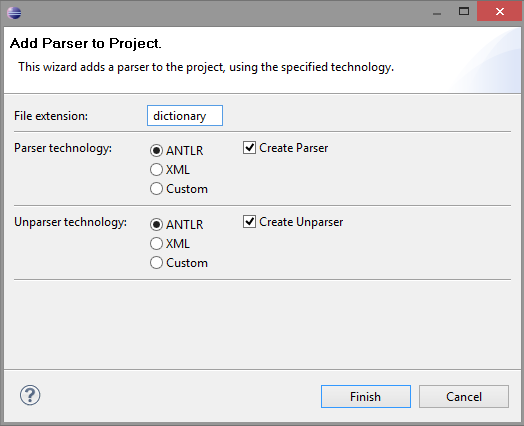
\includegraphics[width=0.6\textwidth]{pics/moca/2TextToMocaTree/2-AddParser.png}
  \caption{Add Parser/Unparser}
  \label{fig:moca-2-AddParser}
\end{center}
\end{figure}

\end{enumerate}

If everything has been installed and set up properly, parser and unparser stubs should be generated and \texttt{ANTLR} should automatically build the corresponding Java code as depicted in Fig.~\ref{fig:moca-3-WizardResult}. 

%\usepackage{graphics} is needed for \includegraphics
\begin{figure}[!htbp]
\begin{center}
 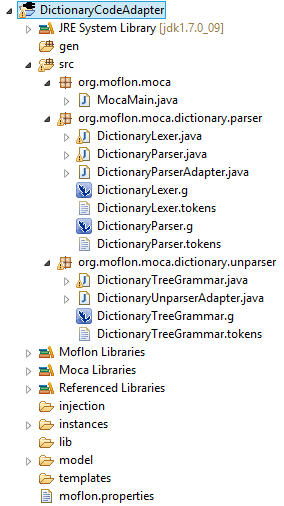
\includegraphics[width=0.6\textwidth]{pics/moca/2TextToMocaTree/3-WizardResult.png}
  \caption{Workspace after wizard finishes}
  \label{fig:moca-3-WizardResult}
\end{center}
\end{figure}
 
 
\section{Text-to-Tree transformation}

As we shall see in a moment, libraries and shelves correspond to a folder structure while the contents for a single dictionary are specified in a file.
Figure \ref{fig:moca-4-Tokens} depicts a small sample of the textual syntax used to specify a dictionary.
On the way to an instance model of our dictionary metamodel, the very first step is to create nice \emph{chunks} of characters.
This step is called \emph{lexing} and it simplifies the actual comprehension of the complete text.
Interestingly human beings actually comprehend text in a similar manner, one recognizes whole words without ``seeing'' every individual character.
This is the reason why you can siltl raed tihs sneentce alsomt eforftlsesly.   
A lexer recognizes these chunks or \emph{tokens} and passes them on as a token stream to the \emph{parser} that does the actual work of recognizing complex hierarchical and recursive structures.   
   
To recognize the tokens as indicated in Fig.~\ref{fig:moca-4-Tokens}, \texttt{ANTLR} can automatically generate a lexer in Java from a compact specification as depicted in Fig.~\ref{fig:moca-6-lexer}.
This is actually a DSL for lexing and is explained in detail in \cite{ANTLR}.
If you do not know what EBNF is and have problems understanding the lexer grammar then make sure you at least go through the documentation on \url{www.antlr.org} or read relevant chapters in \cite{ANTLR}.

%\usepackage{graphics} is needed for \includegraphics
\begin{figure}[!htbp]
\begin{center}
 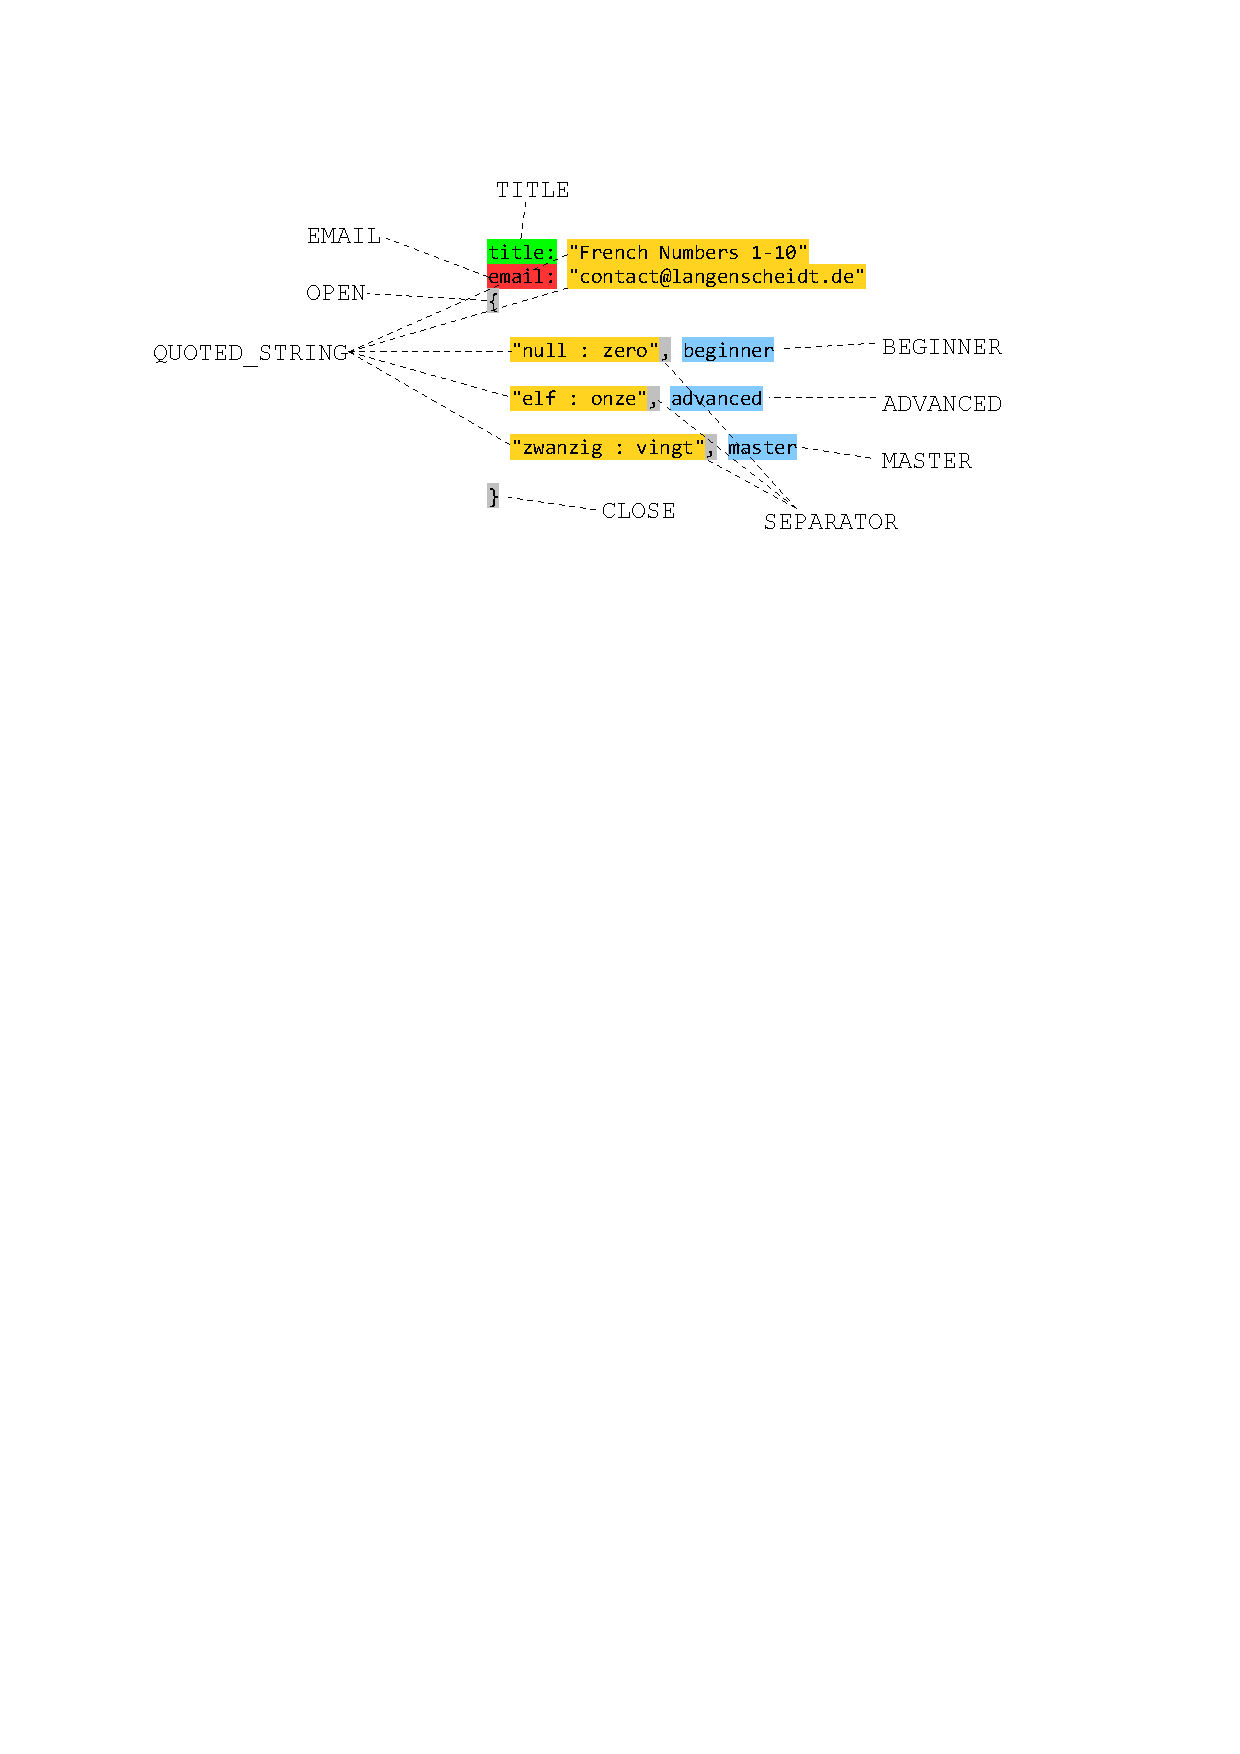
\includegraphics[width=0.7\textwidth]{pics/moca/2TextToMocaTree/4-tokens}
  \caption{Identified tokens in a dictionary file.}
  \label{fig:moca-4-Tokens}
\end{center}
\end{figure}

\begin{enumerate}
\item[$\blacktriangleright$] Edit \texttt{DictionaryLexer.g} so it closely resembles Fig.~\ref{fig:moca-6-lexer}.
Be careful to avoid any typos and mistakes.  Save and make sure it compiles.  
\end{enumerate}

%\usepackage{graphics} is needed for \includegraphics
\begin{figure}[!htbp]
\begin{center}
 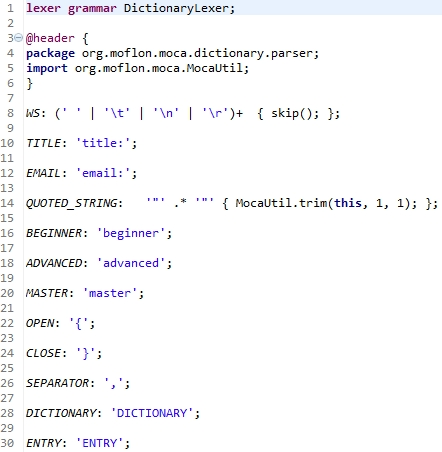
\includegraphics[width=0.65\textwidth]{pics/moca/2TextToMocaTree/6-lexer}
  \caption{Lexer grammar}
  \label{fig:moca-6-lexer}
\end{center}
\end{figure}

The next step is to form the stream of tokens from the lexer into a \emph{tree}.
In this context, a tree is an acyclic, hierarchical, recursive structure as depicted in Fig.~\ref{fig:moca-5-Tree}.
Depending on what the tree is to be used for, it can be organized very differently with extra \emph{structural} nodes like \texttt{DICTIONARY} or \texttt{ENTRY} that were not present in the textual syntax and are used to give additional meaning to the tree. 

%\usepackage{graphics} is needed for \includegraphics
\begin{figure}[htp]
\begin{center}
 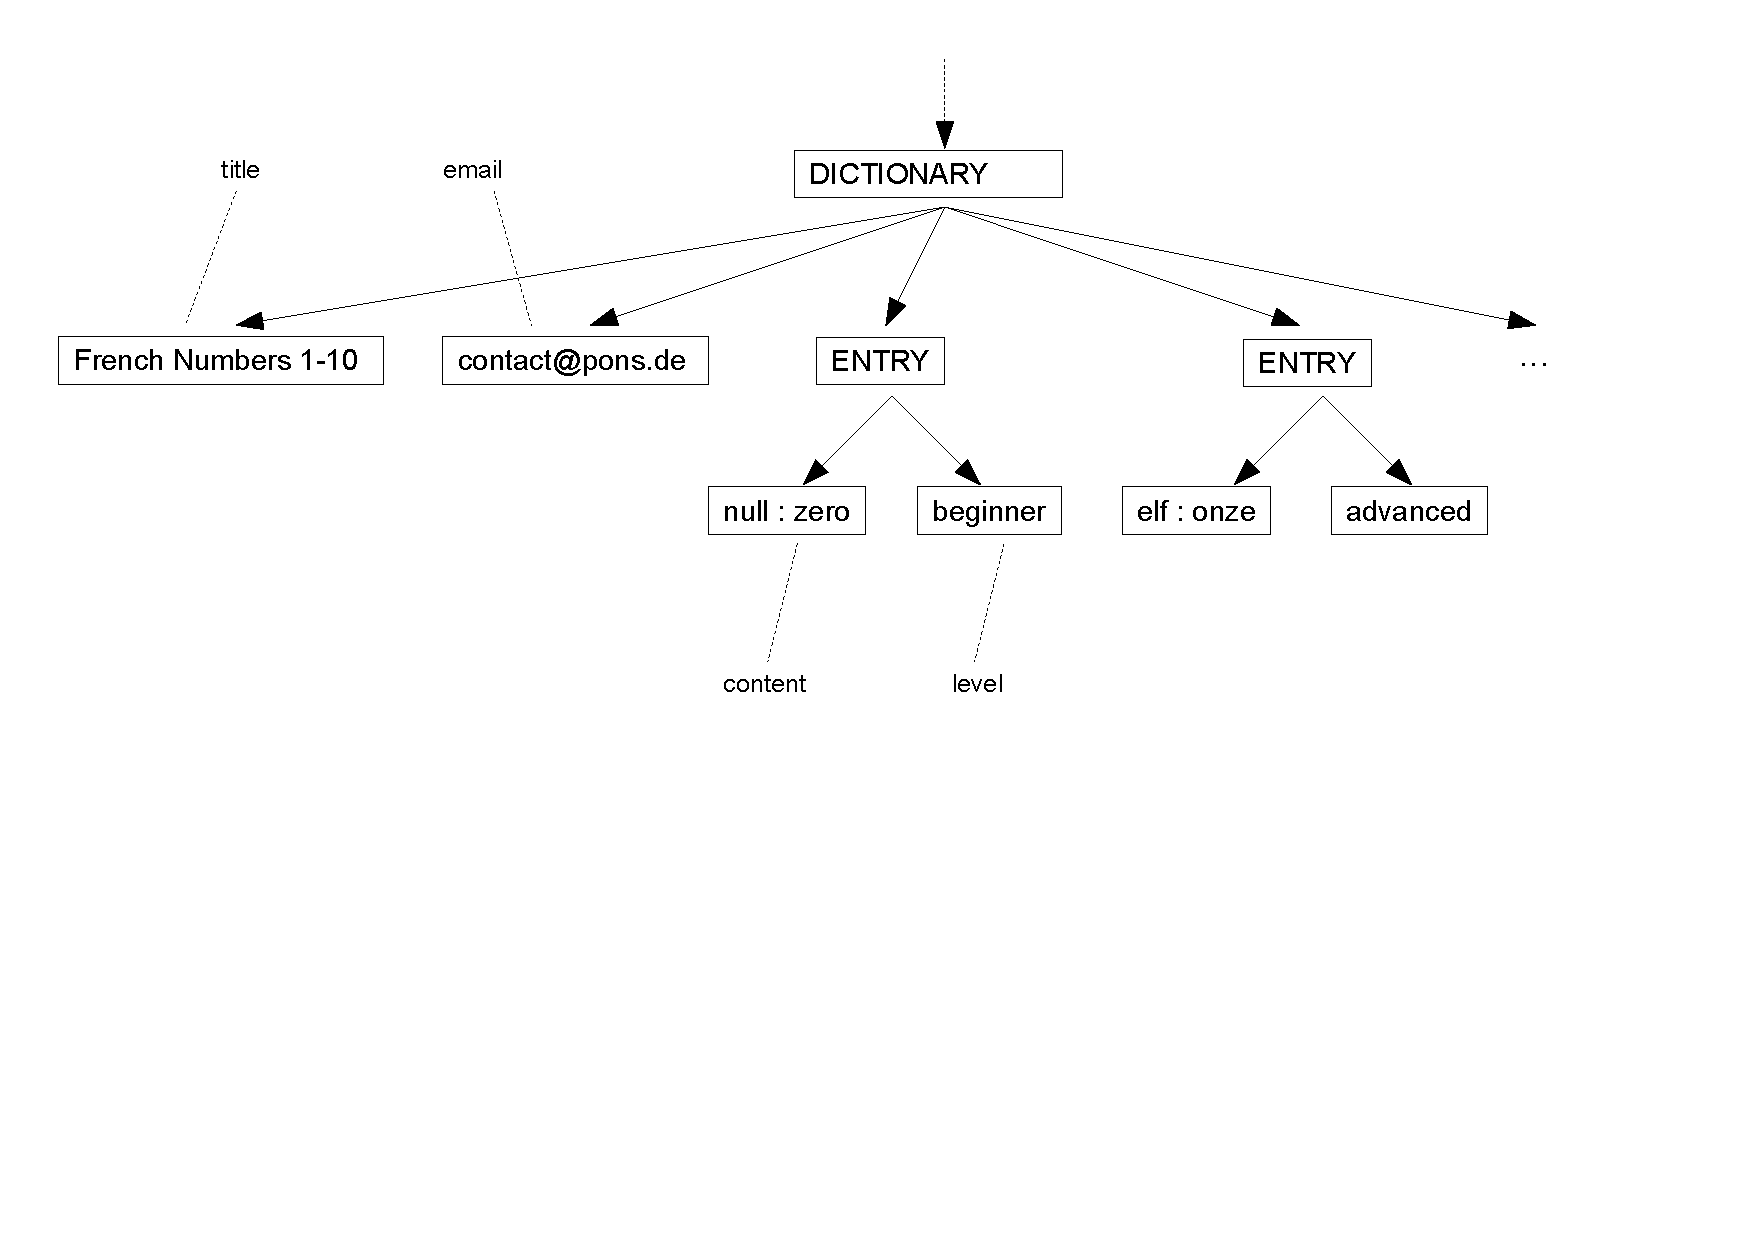
\includegraphics[width=\textwidth]{pics/moca/2TextToMocaTree/5-tree}
  \caption{MocaTree structure}
  \label{fig:moca-5-Tree}
\end{center}
\end{figure}

\begin{enumerate}
\item[$\blacktriangleright$] Edit \texttt{DictionaryParser.g} so it closely resembles Fig.~\ref{fig:moca-7-parser}.
As with the lexer, avoid typos and mistakes and make sure it compiles.
\end{enumerate}

%\usepackage{graphics} is needed for \includegraphics
\begin{figure}[!htbp]
\begin{center}
 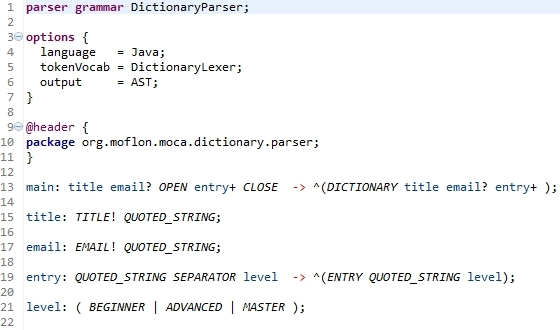
\includegraphics[width=0.9\textwidth]{pics/moca/2TextToMocaTree/7-parser}
  \caption{Parser grammar}
  \label{fig:moca-7-parser}
\end{center}
\end{figure}
The parser grammar is quite similar to the lexer grammar, but there are \emph{parser actions} after the \texttt{->} symbol, which build up the tree.
Using this simple tree language, one can (1) abstract from tokens like \texttt{\{} or \texttt{\}}, which are just \emph{syntactical noise}\footnote{In this context, content that is irrelevant for our model.} and (2) enrich the tree with structural nodes like \texttt{ENTRY}, which add explicit structure to the tree.
Please refer to \cite{ANTLR} and online resources for a detailed explanation of the syntax and semantics of the parser grammar supported by \texttt{ANTLR}. 
 
%\usepackage{graphics} is needed for \includegraphics
\begin{figure}[htp]
\begin{center}
 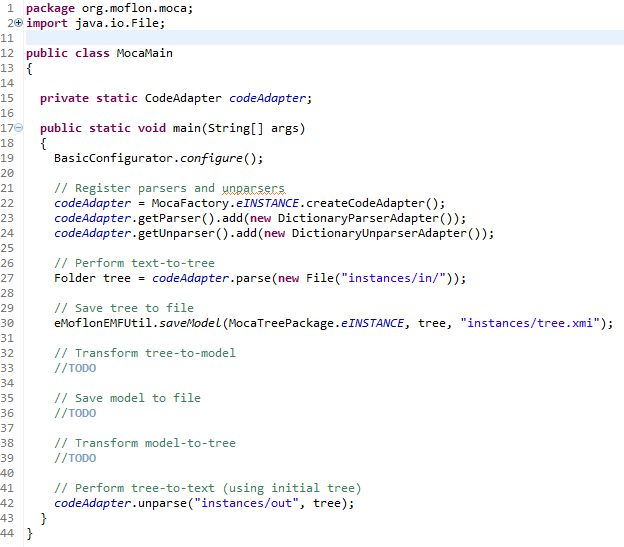
\includegraphics[width=\textwidth]{pics/moca/2TextToMocaTree/8-MocaMain}
  \caption{Generated main method}
  \label{fig:moca-8-MocaMain} 
\end{center}
\end{figure}

Before we take our lexer and parser for a spin, open \texttt{MocaMain.java} and inspect it.
If everything went right it should bear a striking resemblance to Fig.~\ref{fig:moca-8-MocaMain}.
For the moment, please comment out line 24\footnote{If you forget this the default implementation of the unparser will throw an exception.} as we shall define the unparser, i.e., model-to-text a bit later.
Do not change anything else and just note how the parser is added to the Moca framework (line 23) via an adapter (\texttt{Dictionary\-Parser\-Adapter}).
Go ahead and look at what the adapter exactly does.
All the code can be adjusted and used, for example, to define which files the parser is to be used for (per default the adapter registers for \texttt{*.dictionary} files).
The main job of the adapter is to hide \texttt{ANTLR} specifics so the framework remains (parser) technology agnostic.
If you decide to use a different parser generator or write the parser by hand you would need to implement a corresponding adapter from scratch.

On line 27, the input for the framework is set, meaning that all folders in \texttt{./instances/in} are parsed.
In a nutshell, each folder is taken as a root of a tree and the folder and file structure is reflected as a hierarchy of (children) nodes in the tree.
For each file, the framework searches for a registered parser that is responsible for the particular file, passes the content on to the parser and plugs in the tree from the parser as a single subtree of the corresponding file node in the overall tree.  Take a look at Fig.~\ref{fig:moca-overview} again and review the parts we have covered.

The final step is now to prepare some input for the framework:
\begin{enumerate}
  \item[$\blacktriangleright$] Create the directory structure depicted in Fig.~\ref{fig:moca-inputdata} in \texttt{Dictionary\-Code\-Adapter} and enter the contents from Table~\ref{moca-inputdata} for each of the four \texttt{dictionary} files\footnote{You can just copy\&paste right from this PDF file}.
  %\usepackage{graphics} is needed for \includegraphics
\begin{figure}[htp]
\begin{center}
  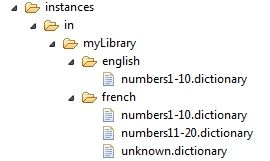
\includegraphics[width=0.5\textwidth]{pics/moca/2TextToMocaTree/inputData}
  \caption{Input directory structure.}
  \label{fig:moca-inputdata}
\end{center}
\end{figure}

\begin{table}
\begin{tabular}{p{6cm} p{6cm} }
\footnotesize
\textbf{english/numbers1-10.dictionary:}
\begin{verbatim}
title: "English Numbers 1-10"
email: "contact@langenscheidt.de"	
{
  "null : zero", beginner
  "eins : one", beginner
  "zwei : two", beginner
  "drei : three", beginner
  "vier : four", beginner
  "fuenf : five", beginner
  "sechs : six", beginner
  "sieben : seven", beginner
  "acht : eight", beginner
  "neun : nine", beginner
  "zehn : ten", beginner 
}
\end{verbatim} 

\textbf{french/numbers1-10.dictionary:}
\begin{verbatim}   
title: "French Numbers 1-10"
email: "contact@pons.de"	
{
  "null : zero", beginner
  "eins : un/une", beginner
  "zwei : deux", beginner
  "drei : trois", beginner
  "vier : quatre", beginner
  "fuenf : cinq", beginner
  "sechs : six", beginner
  "sieben : sept", beginner
  "acht : huit", beginner
  "neun : neuf", beginner
  "zehn : dix", beginner 
}
\end{verbatim}
&

\footnotesize
\textbf{french/numbers11-20.dictionary:}
\begin{verbatim}
title: "French Numbers 11-20"
email: "contact@pons.de"	
{
  "elf : onze", advanced
  "zwoelf : douze", advanced
  "dreizehn : treize", advanced
  "vierzehn : quatorze", advanced
  "fuenfzehn : quinze", advanced
  "sechzehn : seize", master
  "siebzehn : dix-sept", master
  "achtzehn : dix-huit", master
  "neunzehn : dix-neuf", master
  "zwanzig : vingt", master
}

\end{verbatim}
\textbf{french/unknown.dictionary:}
\begin{verbatim}
title: "unknown"
{
  "unbekannt", beginner
}
\end{verbatim}
  \\
\end{tabular}   
\caption{Input files containing dictionaries.}
\label{moca-inputdata}

\end{table}   

\item[$\blacktriangleright$] After creating all the dictionaries, run \texttt{MocaMain.java} as a normal Java application. 
If everything works out right, a file called \texttt{tree.xmi} and an \texttt{out} folder should be created in the \texttt{instances} directory\footnote{You probably have to refresh the \texttt{instances} folder to see the newly created files.}.  
Inspect their contents and compare them to Fig.~\ref{fig:moca-9-ParseResult1}. 
The unparsed files are obviously empty as we haven't implemented an \emph{unparser} yet.  
Don't be irritated by the fact that an \texttt{out/in} is created, this can all be configured in \texttt{MocaMain} but the default assumes \texttt{in} contains multiple folders -- in our case libraries -- and it is therefore treated as the root of the tree.  
One could also unparse directly in \texttt{instances} but the unparsed \texttt{in} would have to be renamed in \texttt{MocaMain}.
\end{enumerate}

%\usepackage{graphics} is needed for \includegraphics
\begin{figure}[!htbp]
\begin{center}
 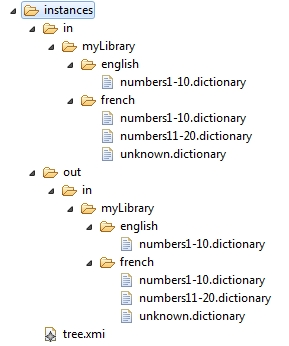
\includegraphics[width=0.4\textwidth]{pics/moca/2TextToMocaTree/9-ParseResult1}
  \caption{Directory \texttt{instances} after parsing}
  \label{fig:moca-9-ParseResult1}
\end{center}
\end{figure} 

\begin{enumerate}
  \item[$\blacktriangleright$] Double-click \texttt{tree.xmi}\footnote{Depending on the plugins you have installed, you might have to explicitly choose \texttt{Open With/Sample Reflective Ecore Model Editor}.} and compare the contents to Fig.~\ref{fig:moca-10-ParseResult2}. At this point, you can reflect on the structure of the tree and note the directory structure, file nodes and the subtrees from the parser.
  
This is important to understand; the directory structure is transformed to a corresponding hierarchy of \texttt{Folders} and \texttt{Files}.
The actual \emph{textual content} of each file is then transformed to a subtree using a registered, suitable parser.
The resulting subtree from the parser is then plugged into the tree by setting its root as the single child node of a \texttt{File}.
%\usepackage{graphics} is needed for \includegraphics
\begin{figure}[!htbp]
\begin{center}
 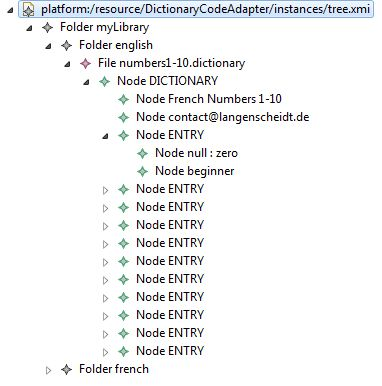
\includegraphics[width=0.55\textwidth]{pics/moca/2TextToMocaTree/10-ParseResult2}
  \caption{MocaTree created by the framework using our parser}
  \label{fig:moca-10-ParseResult2}
\end{center}
\end{figure}
\end{enumerate}

If everything worked out then well done!  We now have a nice tree that we can work on with SDMs and transform in a few simple steps to an actual instance of our Dictionary metamodel.

\section{Tree-to-Model transformation with SDMs}

The next step is to specify a set of SDMs to transform our tree to an instance of our dictionary metamodel.
Take a look at the overview (Fig.~\ref{fig:moca-overview}) again and try to identify which arrow depicts exactly this \emph{tree-to-model} transformation.
Just a short comment;  all SDMs in this section depict story patterns directly in their story nodes.
Please do not take this as a \emph{best practice}, in fact we actually recommend always extracting story patterns.
It's just easier for the tutorial to fit each SDM on a single page!

\begin{enumerate}
  \item[$\blacktriangleright$]  In the code adapter project
  \texttt{DictionaryCodeAdapter}, create a \texttt{Trans\-for\-mer} class with the methods and references to the \texttt{Library} class as depicted in Fig.~\ref{fig:moca-DictionaryCodeAdapter}.\footnote{Do not forget to hold \texttt{Ctrl} when dragging the class in and to choose ``as Simple Link'' so that the class itself is added to the diagram and not an instance of it.}
  Some of the methods are for the model-to-text transformation and the corresponding SDMs shall be handled in Chapter~\ref{chap:model-to-tree}.
%\usepackage{graphics} is needed for \includegraphics
\begin{figure}[!htbp]
\begin{center}
 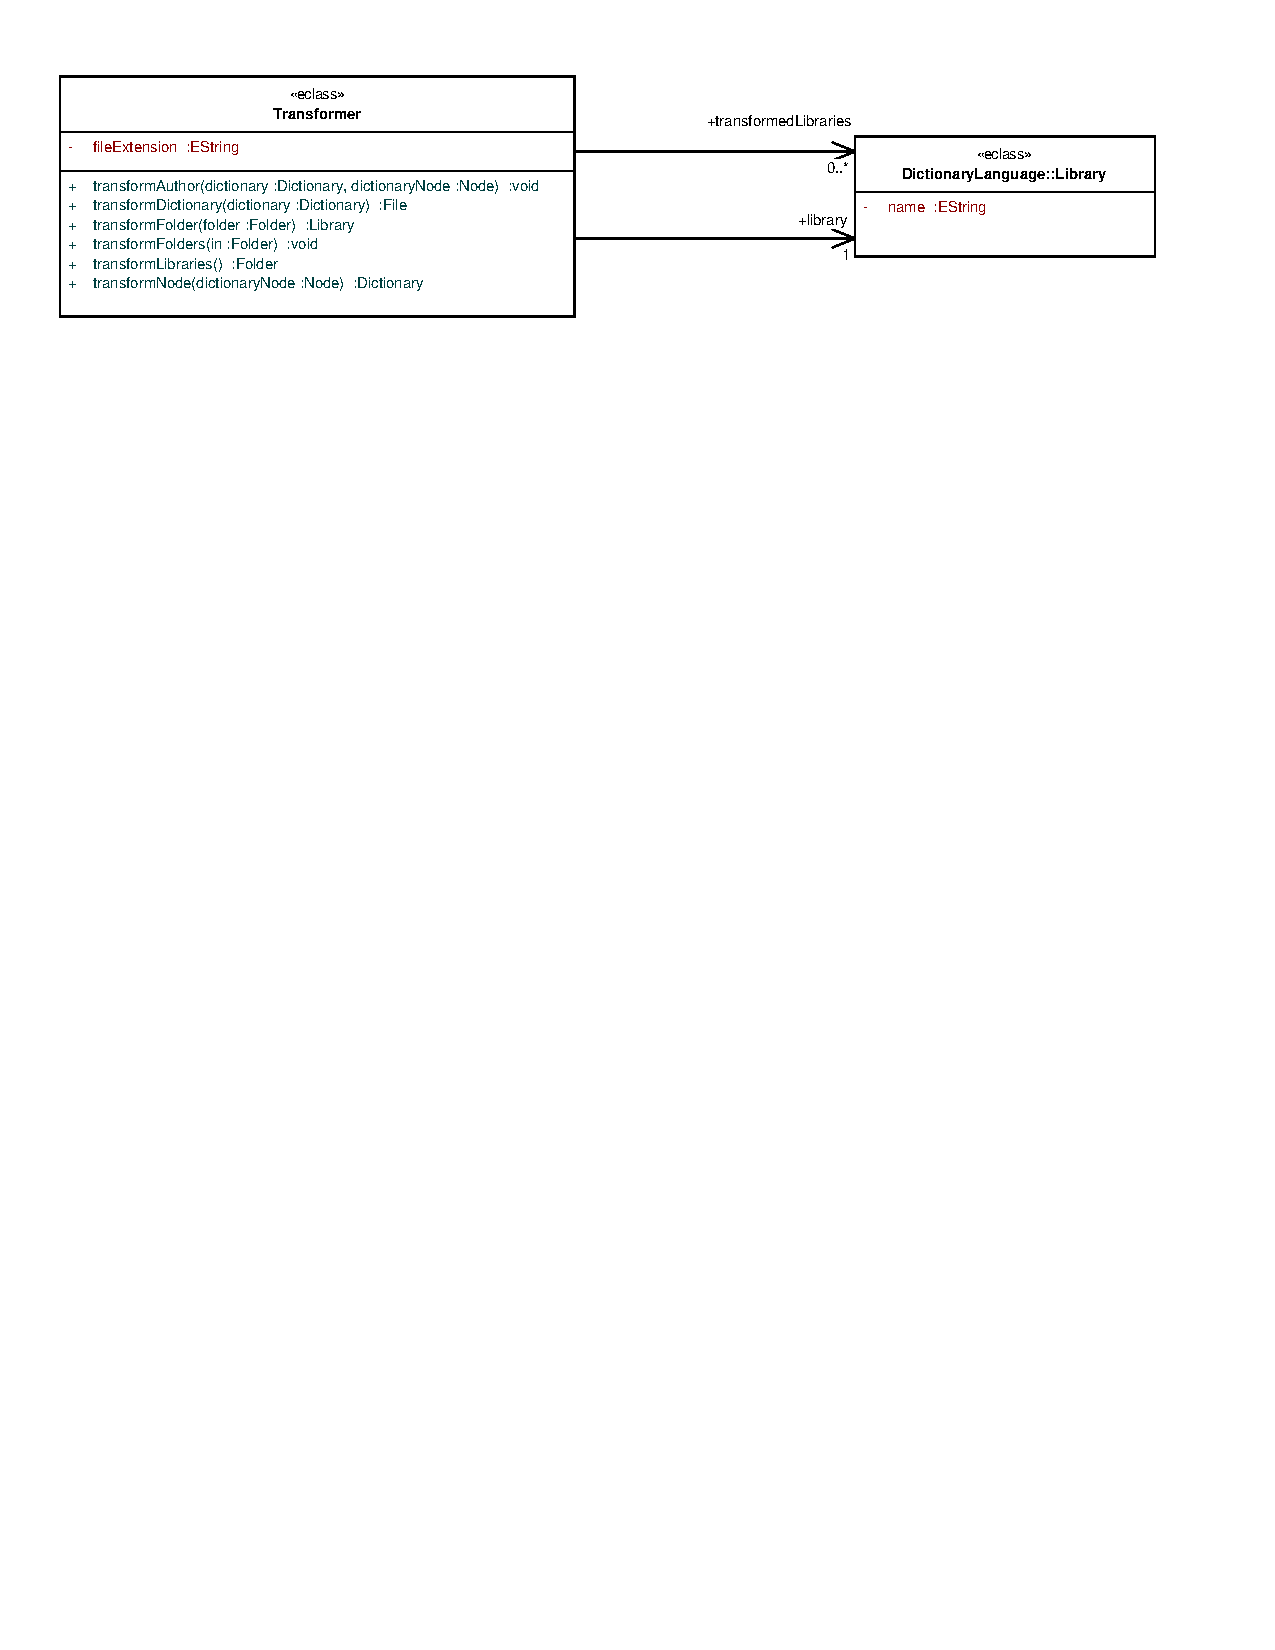
\includegraphics[width=\textwidth]{pics/moca/3MocaTreeToModel/DictionaryCodeAdapter}
  \caption{Transformer class with methods for SDMs}
  \label{fig:moca-DictionaryCodeAdapter}
\end{center}
\end{figure}
\item[$\blacktriangleright$] The first SDM \texttt{transformFolders(Folder)~:void} (Fig.~\ref{fig:moca-transformFolders}) simply iterates through all the library folders and stores the created libraries in the collection \texttt{transformedLibraries}.
%\usepackage{graphics} is needed for \includegraphics
\begin{figure}[!htbp]
\begin{center}
 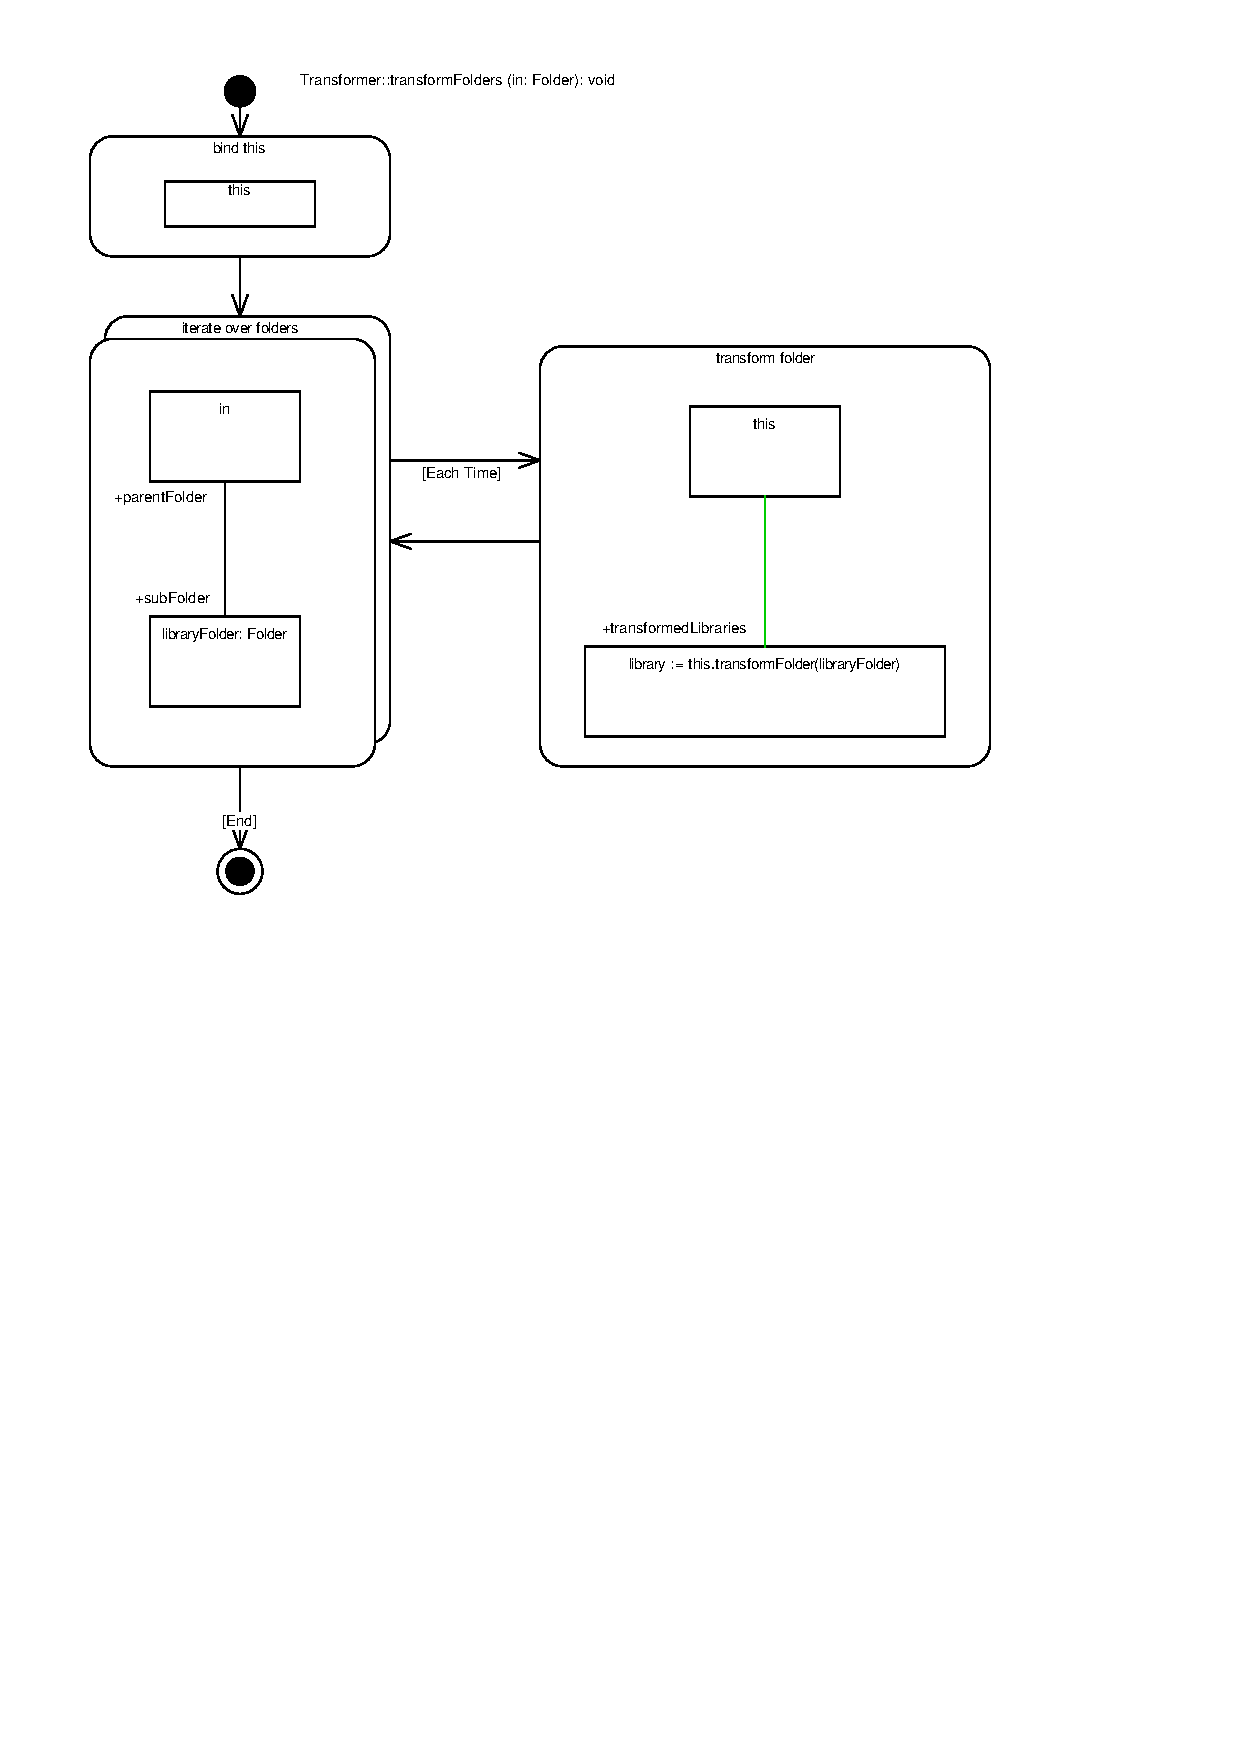
\includegraphics[width=\textwidth]{pics/moca/3MocaTreeToModel/transformFolders}
  \caption{Iterate over all subfolders of the given folder}
  \label{fig:moca-transformFolders}
\end{center}
\end{figure}
\item[$\blacktriangleright$]  \texttt{transformFolder(Folder)~:Library} (Fig.~\ref{fig:moca-transformFolder}) does the main work and creates a corresponding library with shelves for the given folder, delegating the actual creation of dictionaries to \texttt{transformNode}.
The SDM uses features that we have treated in previous chapters.

\clearpage
Note that the exogenous transformation is specified by simply drag \& dropping in elements from \emph{different} metamodels as required!
All dependencies are automatically added when exporting to Eclipse -- now isn't that as simple as ABC?
%\usepackage{graphics} is needed for \includegraphics
\begin{figure}[!htbp]
\begin{center}
 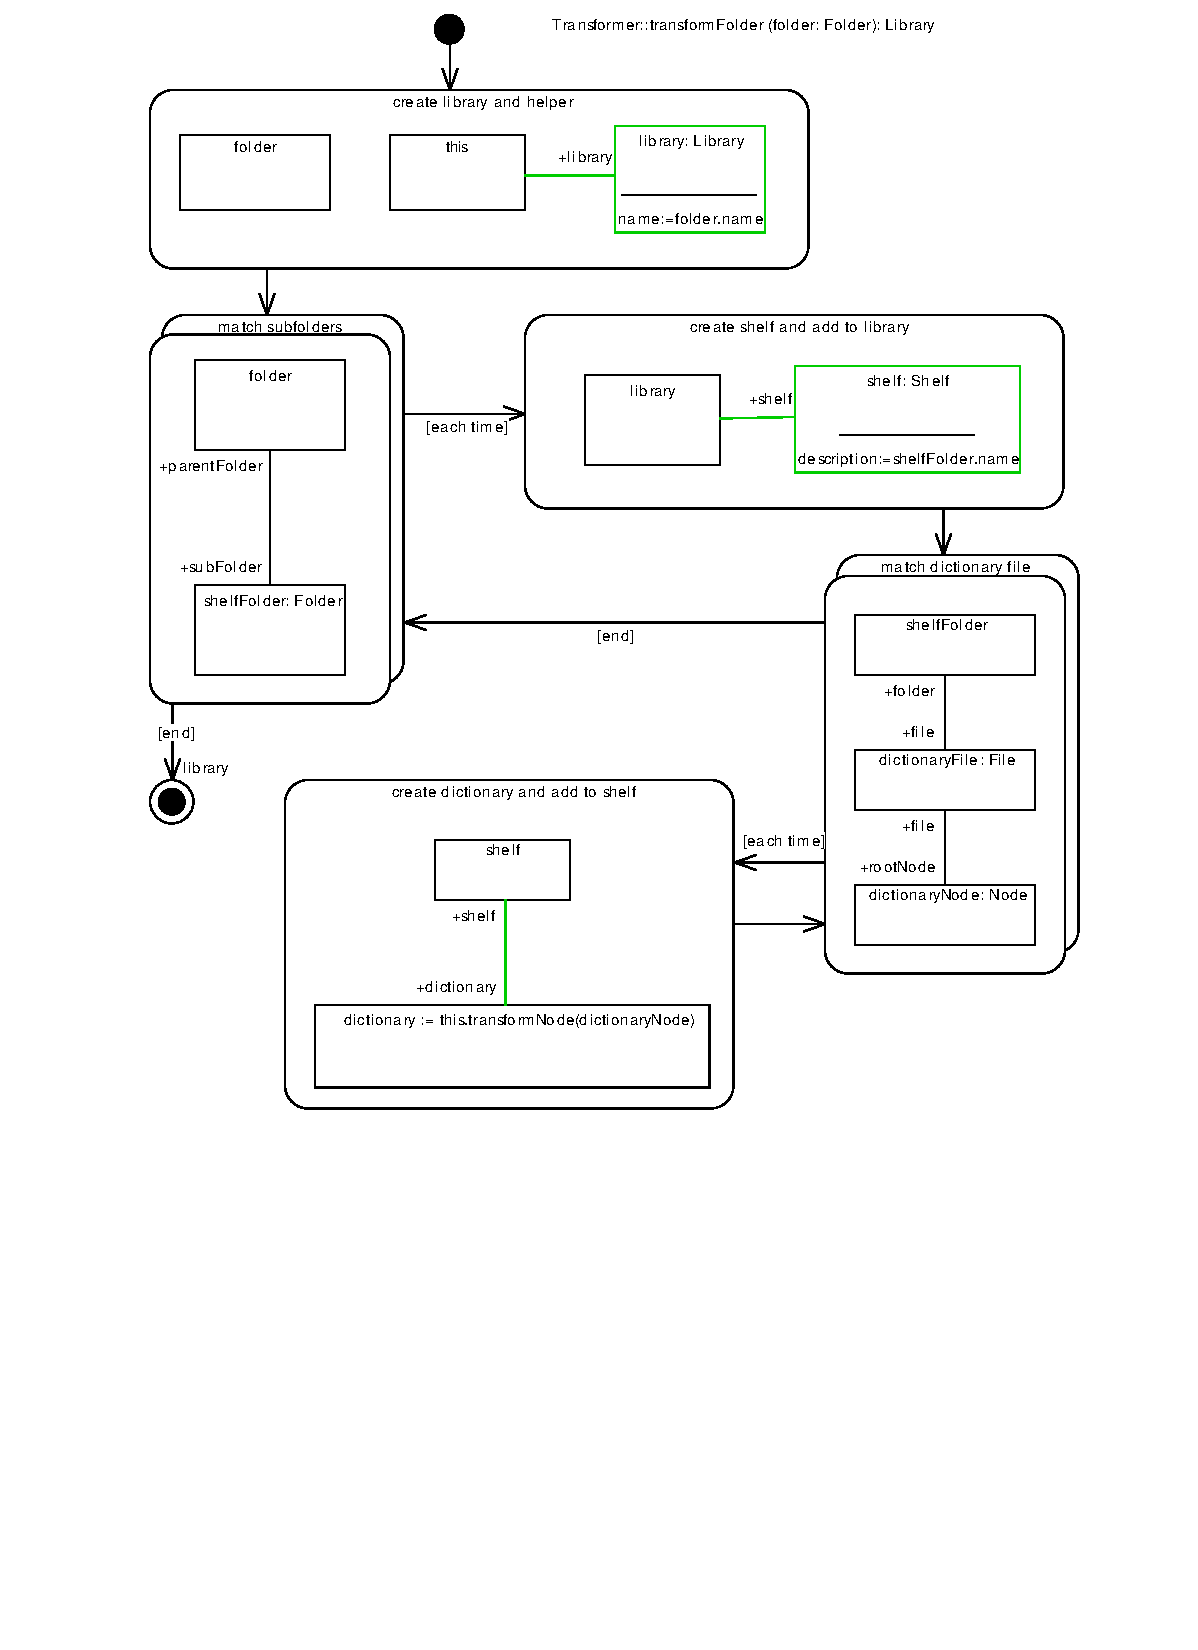
\includegraphics[width=\textwidth]{pics/moca/3MocaTreeToModel/transformFolderPrintPdf}
  \caption{Transforming the outermost folder into a library}
  \label{fig:moca-transformFolder}
\end{center}
\end{figure}

\clearpage

\item[$\blacktriangleright$] The next SDM, \texttt{transformNode(Node)~:Dic\-tion\-ary} (Fig.~\ref{fig:moca-transformNode}) takes a node, representing a dictionary, and builds up a dictionary object, adding entries appropriately.
It further delegates creation of authors to \texttt{transformAuthor}.\footnote{Note that multiple arguments for a MethodCallExpression \emph{cannot} be entered on a single line and separated, e.g. with a ``,'' but rather have to be chosen in the drop-down menu and entered separately, pressing \texttt{Save} each time.}
Note how \emph{indices} are used in the story node \texttt{match entry node} to decide, according to convention (how we built the tree), which node in the tree is to be interpreted as content and which as the level of the entry.
%\usepackage{graphics} is needed for \includegraphics
\begin{figure}[!htbp]
\begin{center}
 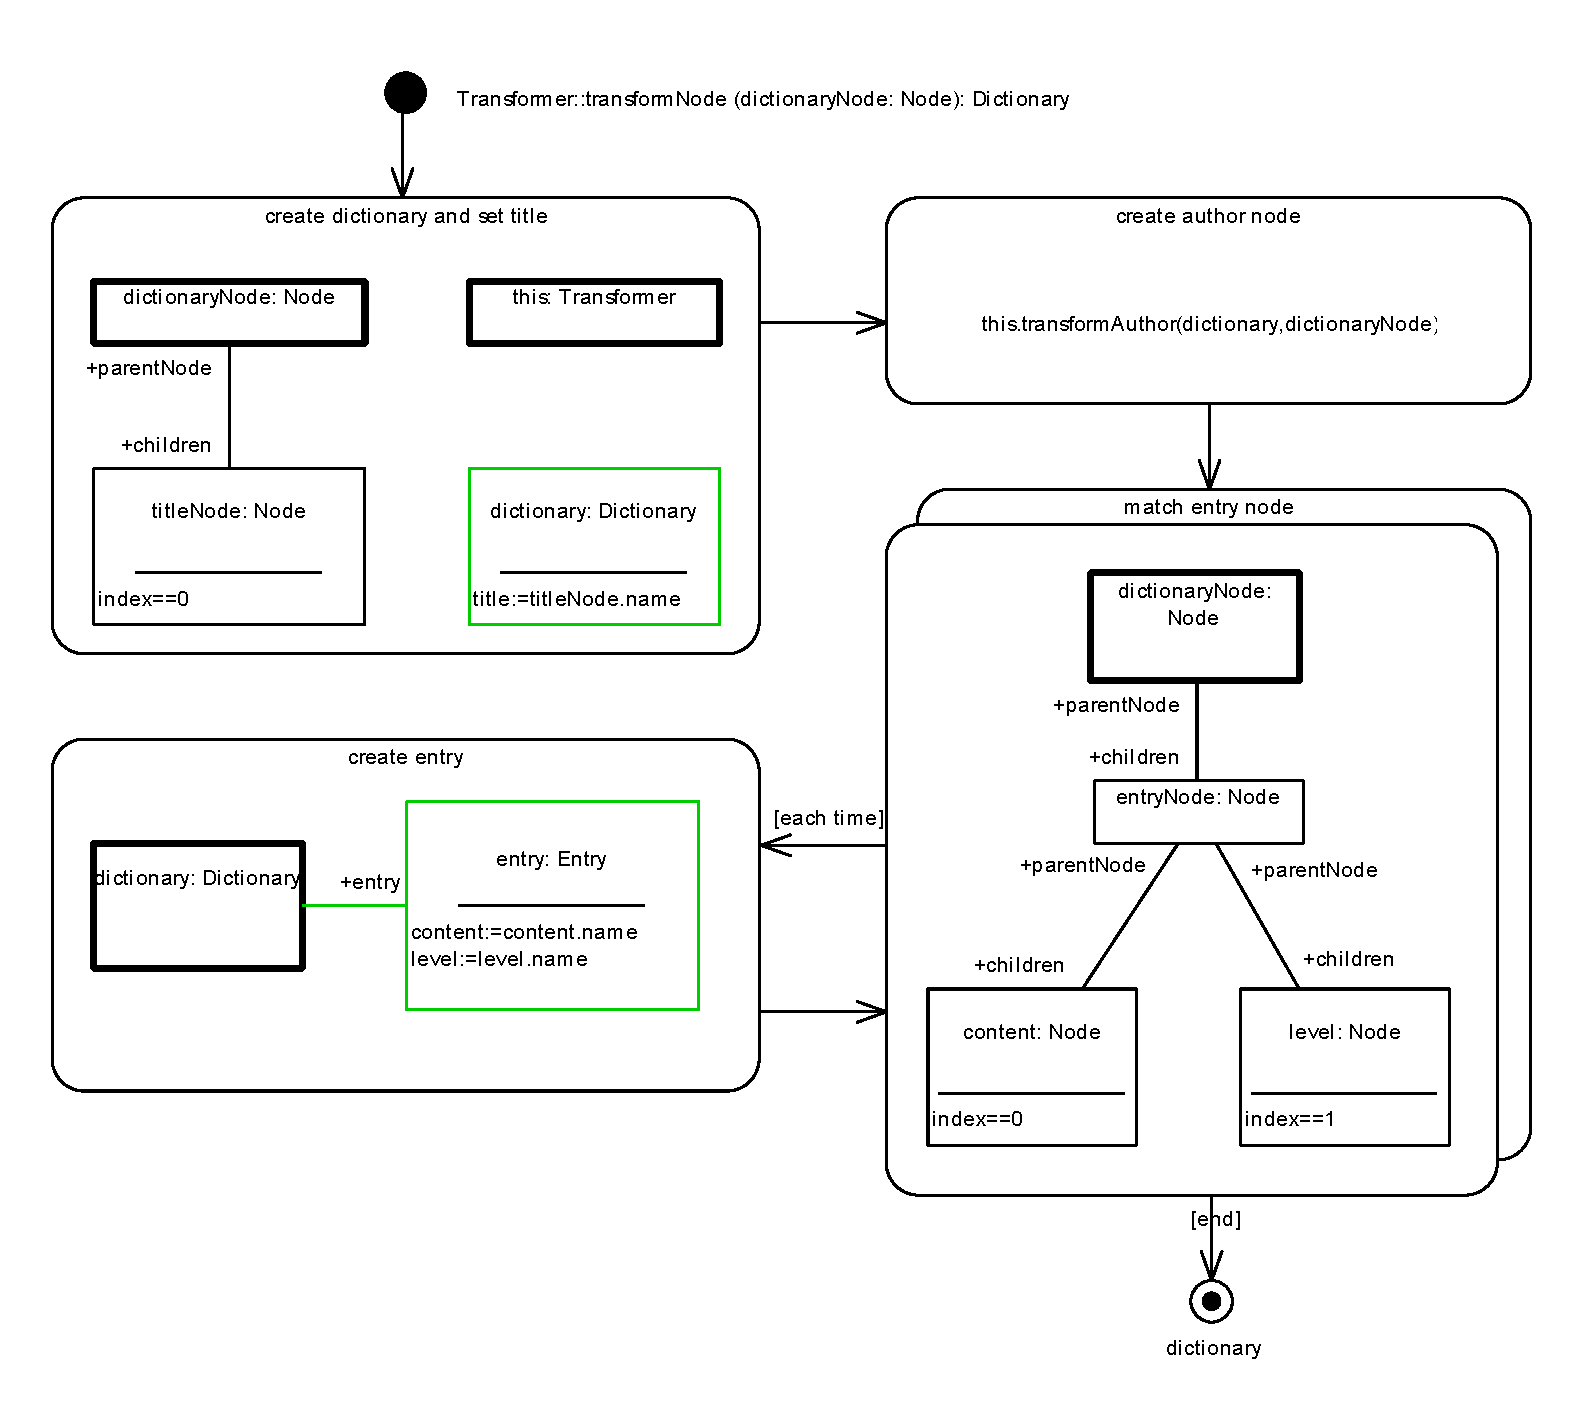
\includegraphics[width=\textwidth]{pics/moca/3MocaTreeToModel/transformNodePrintPdf}
  \caption{Creating dictionaries from dictionary nodes} 
  \label{fig:moca-transformNode}
\end{center}
\end{figure}

\item[$\blacktriangleright$] To wrap things up, create the last SDM, \texttt{trans\-form\-Author(Node)} as depicted in Fig.~\ref{fig:moca-transformAuthor}.
This SDM checks in \texttt{match author node} if the node with \texttt{index} 1 is \emph{not} an entry.
Again according to convention, this would be an author node which is optional.
If no such node exists we do not create an author and simply return.
If such a node does exist, a further complication is that the author might already be known in the library.
In order to avoid multiple, actually identical authors, the author object variable in \texttt{create author} is set to \texttt{optional} and to \texttt{create}.
\marginpar{\emph{Optional Create}} 
 
The semantics of \emph{optional create} is the following:  if a match for the object variable with the specified attribute \emph{constraints} is found, it is used.
If no match can be found then the object variable is created and the specified attribute assignments are carried out.

This is exactly how we need to handle authors -- cool right? 
%\usepackage{graphics} is needed for \includegraphics
\begin{figure}[!htbp]
\begin{center}
 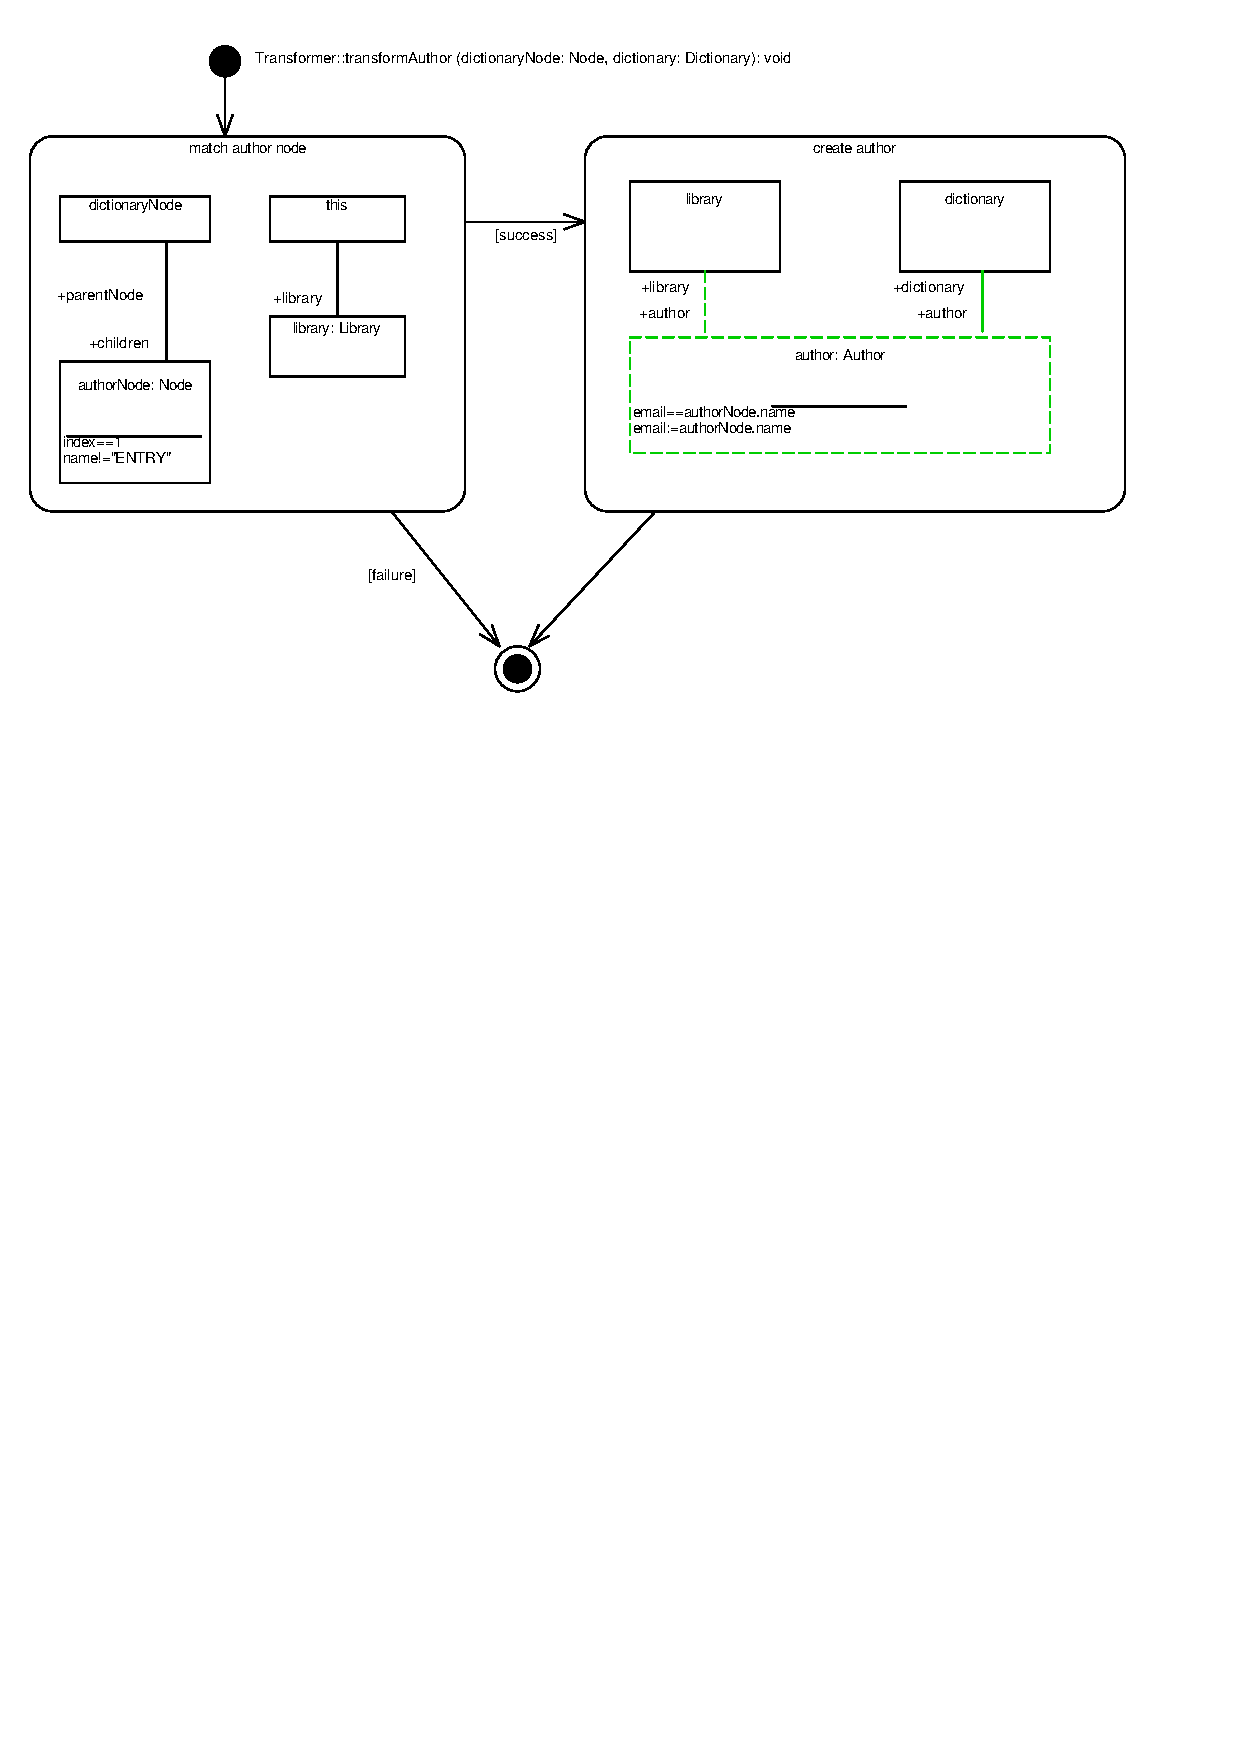
\includegraphics[width=\textwidth]{pics/moca/3MocaTreeToModel/transformAuthorPrint}
  \caption{Handling Authors}
  \label{fig:moca-transformAuthor}
\end{center}
\end{figure}

\item[$\blacktriangleright$] As a final step, open \texttt{MocaMain.java}
(Fig.~\ref{fig:moca-8-MocaMain}) and edit lines 32 -- 36 as follows:
\begin{verbatim}
// Perform tree-to-model 
Transformer transformer = DictionaryCodeAdapterFactory.
  eINSTANCE.createTransformer();
transformer.transformFolders(tree);

// Save library models
for (Library library : transformer.getTransformedLibraries())
  eMoflonEMFUtil.saveModel(library, 
    "instances/" + library.getName() + ".xmi"); 
\end{verbatim}
  
To see the effects of running \texttt{MocaMain.java}, refresh (\texttt{F5}) the Eclipse project to see the newly created \texttt{myLibrary.xmi} (Fig.~\ref{fig:moca-created-libary}).  
Open and inspect the library model using the reflective model browser and note especially the cross-tree references between authors and their dictionaries. 
\end{enumerate}

%\usepackage{graphics} is needed for \includegraphics
\begin{figure}[htp]
\begin{center}
  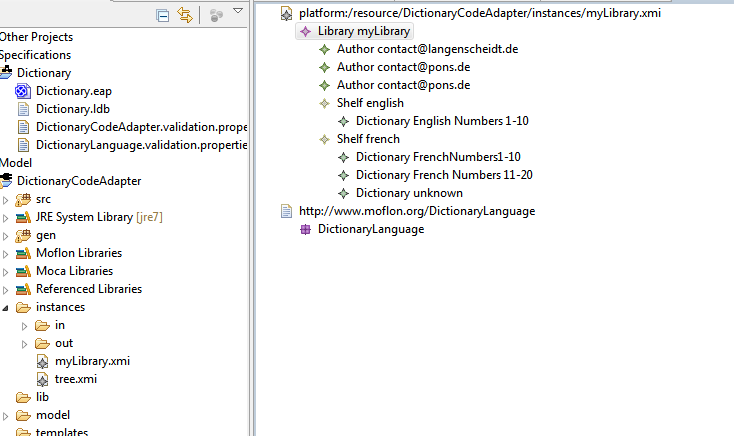
\includegraphics[width=\textwidth]{pics/moca/3MocaTreeToModel/tree_to_model_filesystem.png}
  \caption{Created library model}
  \label{fig:moca-created-libary}
\end{center}
\end{figure}

\section{Model-to-Tree Transformation with SDMs}
\label{chap:model-to-tree}
Do you remember that our unparsed files are still all empty (Fig.~\ref{fig:moca-9-ParseResult1})?
Well it's time to fix that - we need a \emph{model-to-text} transformation to convert library instances to a folder structure with dictionary files in our DSL.
Just like the \emph{text-to-model} transformation, we shall take the same approach of breaking the job into two simpler steps:  a \emph{model-to-tree} transformation  with SDMs (discussed in this chapter) and a \emph{tree-to-text} transformations using ANTLR and a set of templates (discussed in Chapter~\ref{chap:tree-to-text}).
To remind you of the big picture, take a look at Fig.~\ref{fig:moca-overview} and try to figure out where we are right now.

The following SDMs implement the model-to-tree transformation and transform a set of libraries to a single folder with a subfolder per library:
\begin{enumerate}    
\item[$\blacktriangleright$] \texttt{transformLibraries()~:Folder} (Fig.~\ref{fig:moca-transformLibraries}) iterates through all libraries, shelves and dictionaries, creating the appropriate folder structure in the process.
The actual transformation of each dictionary to a file is delegated using a binding expression (a method-call expression).    
  %\usepackage{graphics} is needed for \includegraphics
\begin{figure}[!htbp]
\begin{center}
 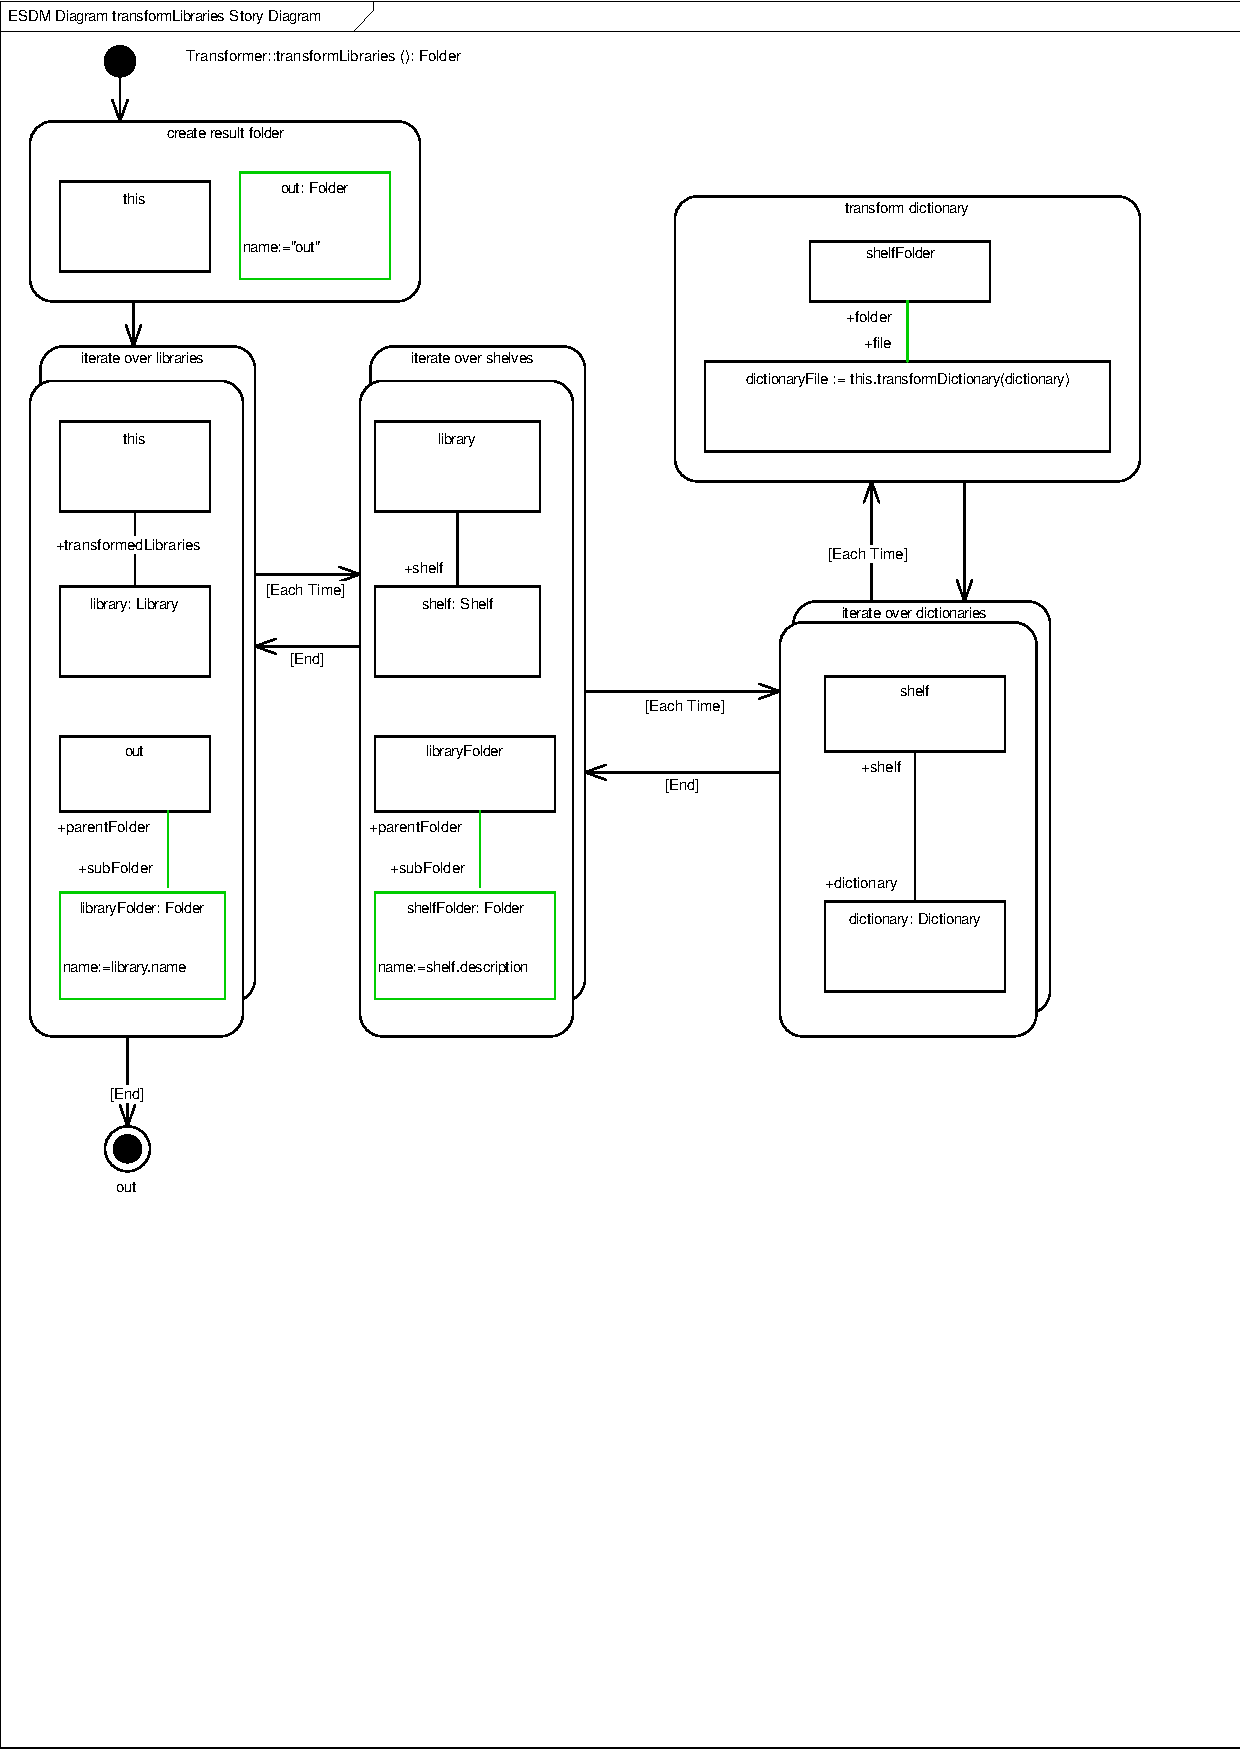
\includegraphics[width=\textwidth]{pics/moca/4ModelToMocaTree/transformLibraries}
  \caption{Iterate over all libraries, shelves and dictionaries} 
  \label{fig:moca-transformLibraries}
\end{center}
\end{figure}

\item[$\blacktriangleright$] \texttt{transformDictionary(Dictionary)~:File} (Fig.~\ref{fig:moca-transformDictionary})\footnote{Please note that the right-hand side of the attribute assignment in \texttt{dictionaryFile} is a literal expression.} does the actual work of transforming a dictionary to a file, handling authors as an optional node in the file subtree.
  %\usepackage{graphics} is needed for \includegraphics
\begin{figure}[!htbp]
\begin{center}
 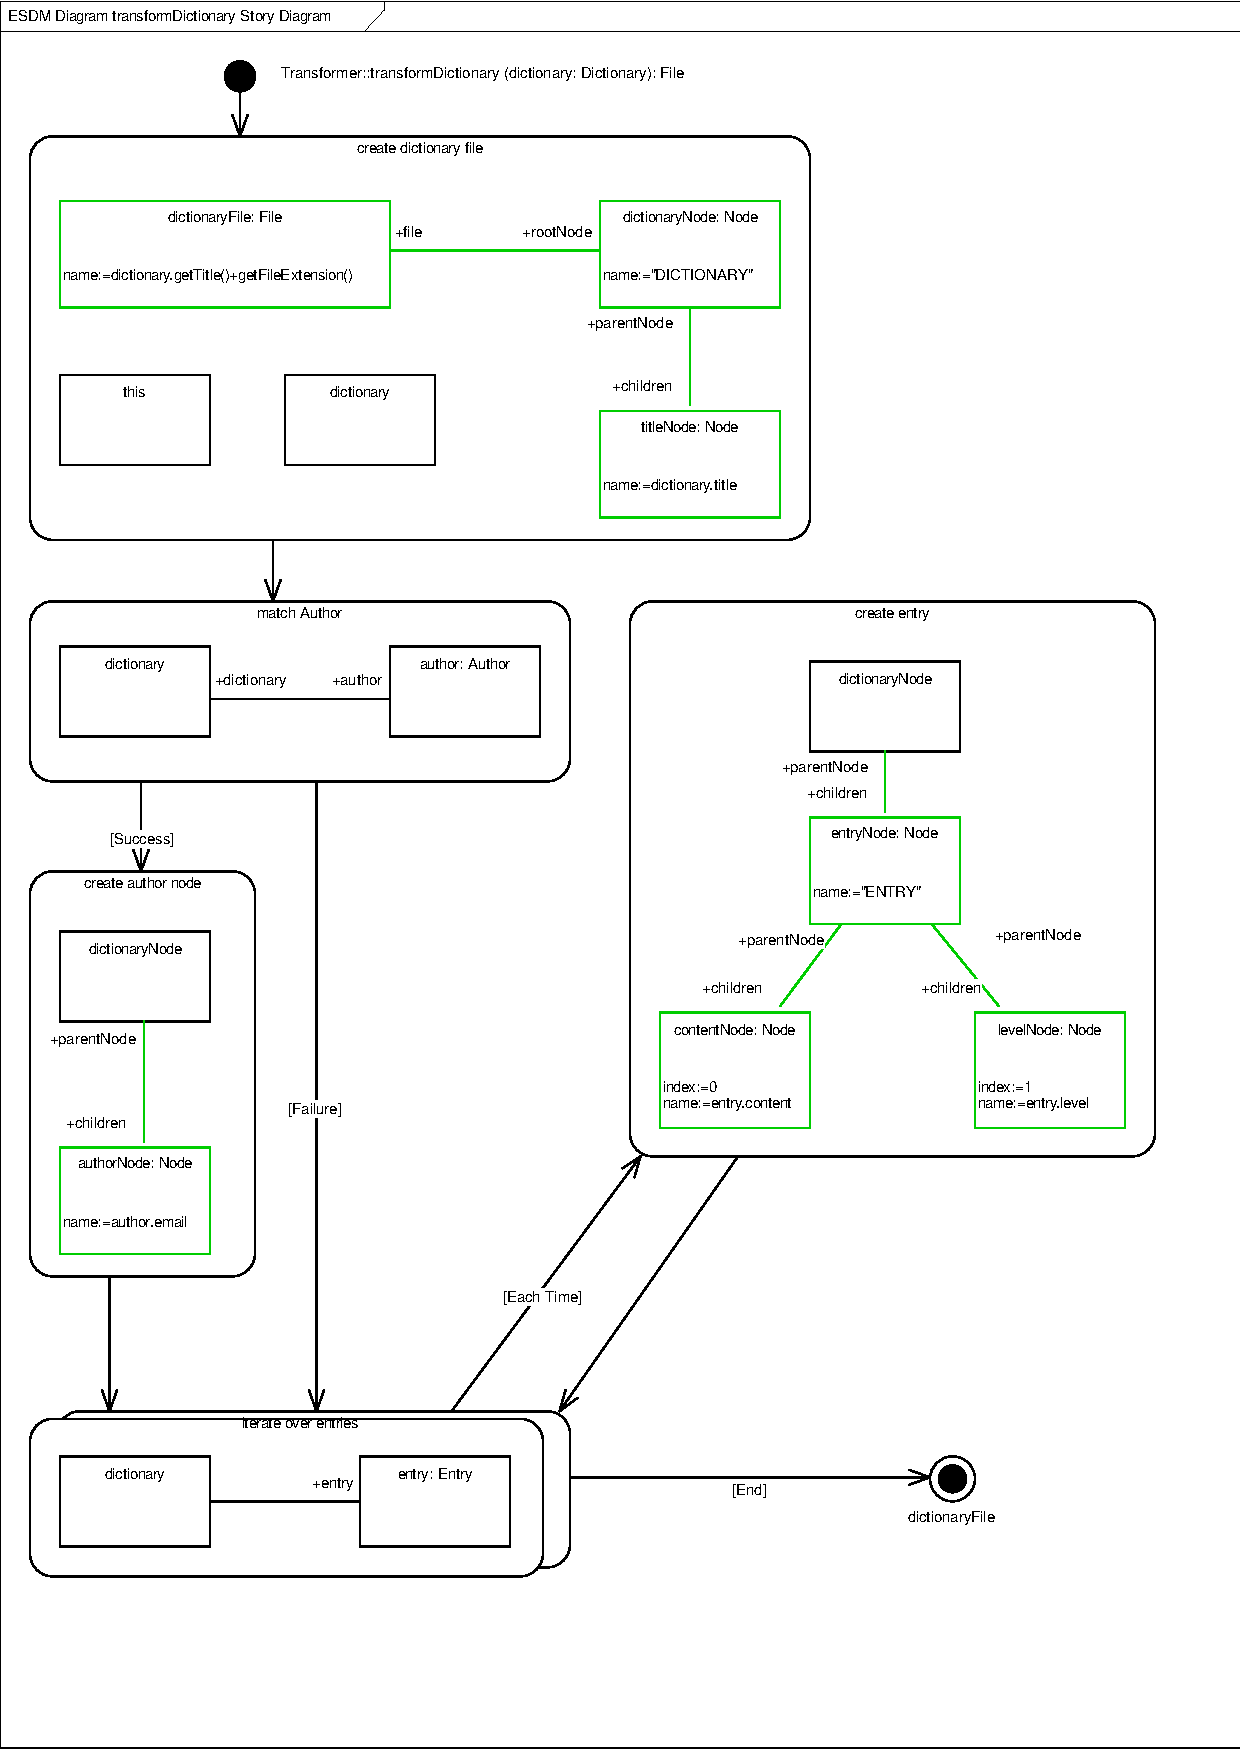
\includegraphics[width=\textwidth]{pics/moca/4ModelToMocaTree/transformDictionary}
  \caption{Create a file from a dictionary with an optional author} 
  \label{fig:moca-transformDictionary}
\end{center}
\end{figure}
\item[$\blacktriangleright$] To invoke the model-to-tree transformation, open \texttt{MocaMain.java} (Fig.~\ref{fig:moca-8-MocaMain}) and edit lines 38-39 as follows.
\begin{verbatim}
// Perform model-to-tree transformation
transformer.setFileExtension(".dictionary");
Folder out = transformer.transformLibraries();
\end{verbatim}
The tree \texttt{out} can of course be persisted to file using \texttt{eMoflonUtil\-.save\-Model} if you wish to inspect it before continuing.
If you did everything right, it should resemble Fig.~\ref{fig:moca-10-ParseResult2} very closely. 
\end{enumerate}

\section{Tree-To-Text Transformation with SDMs}
\label{chap:tree-to-text}

In this last step, we are going to transform our tree to an actual folder structure with files containing text.
One of the coolest things about ANTLR is that the same parser technology can be used to \emph{unparse} a tree.
Analogously to parsing text with a lexer and parser grammar to produce a tree, a tree can be unparsed to text using a \emph{tree grammar} and templates.
\begin{enumerate}
\item[$\blacktriangleright$] Open \texttt{src/org.moflon.org/dictionary/unparser/Dictionary\-Tree\-Grammar.g} (Fig.~\ref{fig:moca-3-WizardResult}), and edit the contents of the file as depicted in Fig.~\ref{fig:moca-DictionaryTreeGrammar}.
A tree grammar is actually very similar to standard EBNF and consists of a set of rules (\texttt{main}, \texttt{entry}) that match a tree fragment (instead of a text fragment) and evaluate a template (instead of building up a tree).
For further details concerning tree grammars we refer to \cite{ANTLR} and the
ANTLR website \url{www.antlr.org}.

  %\usepackage{graphics} is needed for \includegraphics
\begin{figure}[!htbp]
\begin{center}
 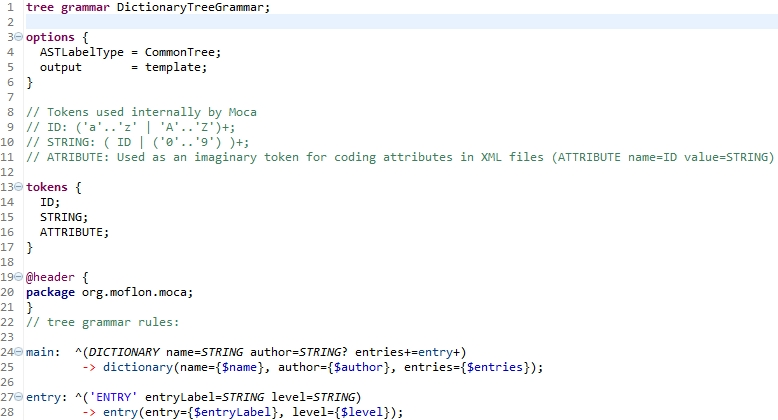
\includegraphics[width=\textwidth]{pics/moca/5MocaTreeToText/DictionaryTreeGrammar}
  \caption{Tree Grammar for the dictionary DSL} 
  \label{fig:moca-DictionaryTreeGrammar}
\end{center}
\end{figure} 

\item[$\blacktriangleright$] In the generated \texttt{src/org.moflon.org/dictionary/unparser/Dic\-tion\-ary\-Unparser\-Adapter.java} (Fig.~\ref{fig:moca-3-WizardResult}) a method for retrieving a group of templates has to be implemented.
Figure \ref{fig:moca-DictionaryUnparserAdapter} depicts the generated version showing how to use either a folder containing different template files, or a single file that contains all templates.
The latter is better for numerous smaller templates, while the former makes sense when the templates contain a lot of static text.
%\usepackage{graphics} is needed for \includegraphics
\clearpage 
\begin{figure}[!htbp]
\begin{center}
 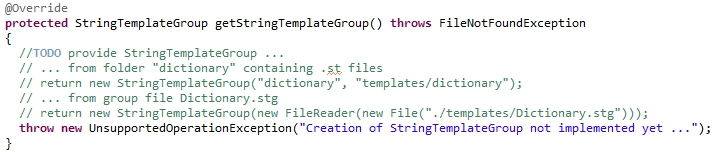
\includegraphics[width=0.87\textwidth]{pics/moca/5MocaTreeToText/UnparserAdapterNotImplemented}
  \caption{Unimplemented method getStringTemplateGroup} 
  \label{fig:moca-DictionaryUnparserAdapter}
\end{center}
\end{figure} 

For our small example a single file with all the templates is ideal, so uncomment the option for a \emph{group file}.
Your unparser adapter should now closely resemble Fig.~\ref{fig:moca-DictionaryUnparserAdapter}.  
 
\begin{figure}[!htbp]
\begin{center}
 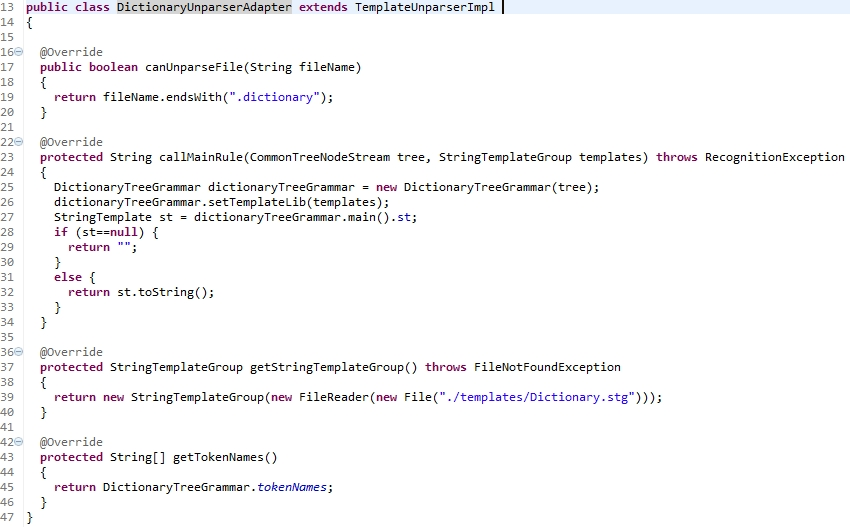
\includegraphics[width=\textwidth]{pics/moca/5MocaTreeToText/UnparserAdapter}
  \caption{Unparser Adapter} 
  \label{fig:moca-DictionaryUnparserAdapter}
\end{center}
\end{figure} 

\item[$\blacktriangleright$] The next step is to create the referenced template group file \texttt{Dic\-tion\-ary.stg} in \texttt{./templates}.
In this file, enter the contents depicted in Fig.~\ref{fig:moca-DictionaryTemplates}.    
ANTLR uses a template language called \emph{StringTemplate}.
StringTemplate is a very simple template language with few constructs and almost no constructs for complicated logic.
This might sound like a disadvantage but it actually prevents you from \emph{programming} in the templates and keeps them simple, readable and easily replaceable.
For further details about StringTemplate we refer to the website \url{www.stringtemplate.org}, a paper that argues for its simplicity \cite{PAR04}, and books on usage and features in combination with ANTLR \cite{ANTLR, LangImplPatterns}.
StringTemplate is pretty intuitive, take a good look at Fig.~\ref{fig:moca-DictionaryTemplates} and pay especially attention to how the templates are invoked in the tree grammar (Fig.~\ref{fig:moca-DictionaryTreeGrammar}).
You can easily make changes in the templates and see how it affects the generated files.
  %\usepackage{graphics} is needed for \includegraphics
\begin{figure}[!htbp]
\begin{center}
 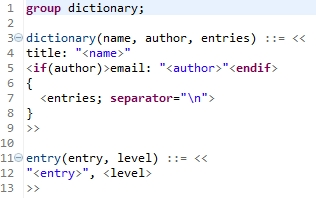
\includegraphics[width=0.5\textwidth]{pics/moca/5MocaTreeToText/DictionaryTemplates}
  \caption{Templates for the Dictionary DSL} 
  \label{fig:moca-DictionaryTemplates}
\end{center}
\end{figure} 

\item[$\blacktriangleright$] To complete the model-to-text transformation, open \texttt{MocaMain.java} (Fig.~\ref{fig:moca-8-MocaMain}) and edit lines 41-42 as follows:
\begin{verbatim}
// Perform tree-to-text
codeAdapter.unparse("instances", out);
\end{verbatim}
This calls the framework method \emph{unparse}, which creates a corresponding folder structure for a MocaTree instance and delegates code generation for each file using the registered unparsers.
This way different unparsers can be registered for different file types (defined by the unparser adapter's \texttt{canUnparseFile} method) and a whole folder structure containing different files can be generated.
Each parser can either use a single template group file like in our case, or a folder containing separated template files.

As we have always been updating our \texttt{MocaMain.java} file incrementally, Fig.~\ref{fig:moca-FinalMocaMain} shows the complete final version so you can compare before trying out the complete text-to-model and model-to-text round trip.

If you have done everything correctly, you should be able to run \texttt{MocaMain} and obtain similar results as depicted in Fig.~\ref{fig:moca-FinalResults}.
Note the created model \texttt{myLibrary.xmi} and the \texttt{.dictionary} files in \texttt{/out} that should now contain appropriate text in our DSL.
As a final test you can manipulate the model directly (e.g., create a new dictionary or shelf, add/delete an author) and adjust \texttt{MocaMain} appropriately so only the model-to-text transformation is performed.
Now compare the generated dictionaries to see if your changes are reflected correctly. 
 
%\usepackage{graphics} is needed for \includegraphics
\begin{figure}[!htbp]
\begin{center}
 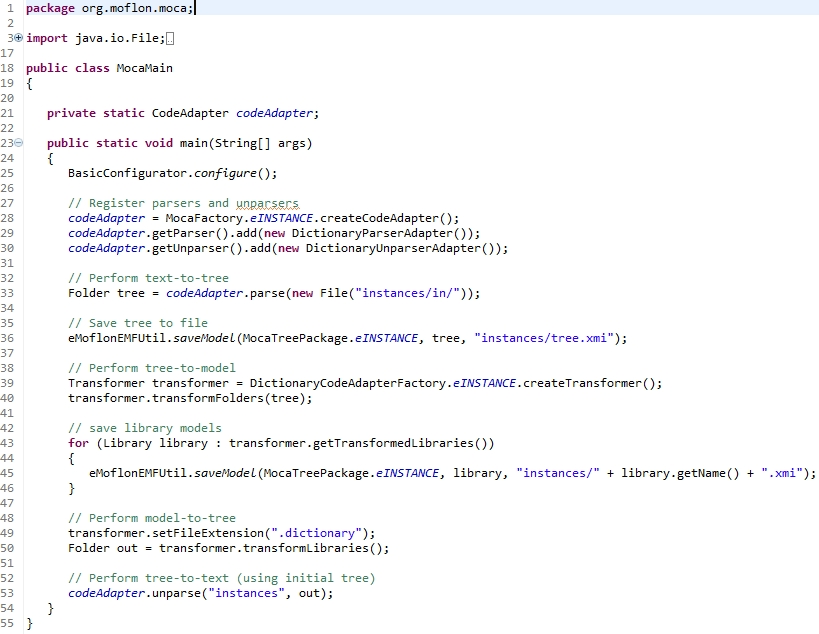
\includegraphics[width=\textwidth]{pics/moca/5MocaTreeToText/MocaMainComplete}
  \caption{Completed main method for Text-to-Model and Model-to-Text} 
  \label{fig:moca-FinalMocaMain}
\end{center}
\end{figure}

%\usepackage{graphics} is needed for \includegraphics
\begin{figure}[!htbp]
\begin{center}
 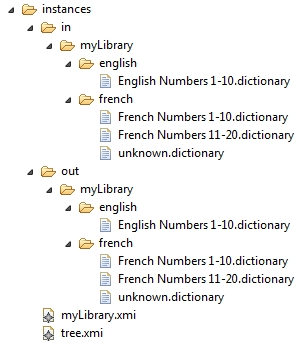
\includegraphics[width=0.5\textwidth]{pics/moca/5MocaTreeToText/InstancesAfterRoundTrip}
  \caption{Directory instances after parsing and unparsing.} 
  \label{fig:moca-FinalResults}
\end{center}
\end{figure}

\end{enumerate}

%\input{mocaHTML}
 
